
\chapter{Imputación de Datos de Tráfico y Contaminación}
\label{chap:eda_imputacion}
\glsresetall

En este capítulo, el lector encontrará el desarrollo del caso de estudio práctico: la imputación de datos de tráfico y contaminación del proyecto Smart Poqueira \citep{smartpoqueira_project}. Comenzaremos describiendo el contexto y los datos. Luego, presentaremos un Análisis Exploratorio (EDA) y detallaremos el entorno experimental, incluyendo el software \texttt{pampaneira\_imputation} y la implementación de los métodos de imputación. Finalmente, se discutirán los resultados de la evaluación.

\section{Infraestructura del Sistema IoT}
\label{sec:contexto_problema}

La infraestructura IoT consta, entre otros sensores, de cámaras con reconocimiento de matrículas \glsp{lpr} estratégicamente ubicadas en los accesos a los municipios de Pampaneira, Bubión y Capileira (Figura~\ref{fig:mapa_fusion}), y una unidad móvil, camión, en el Cementerio Municipal de Pampaneira ($\star$) equipada con sensores para medir diversos contaminantes atmosféricos y variables meteorológicas.

\begin{figure}[H]
    \centering
    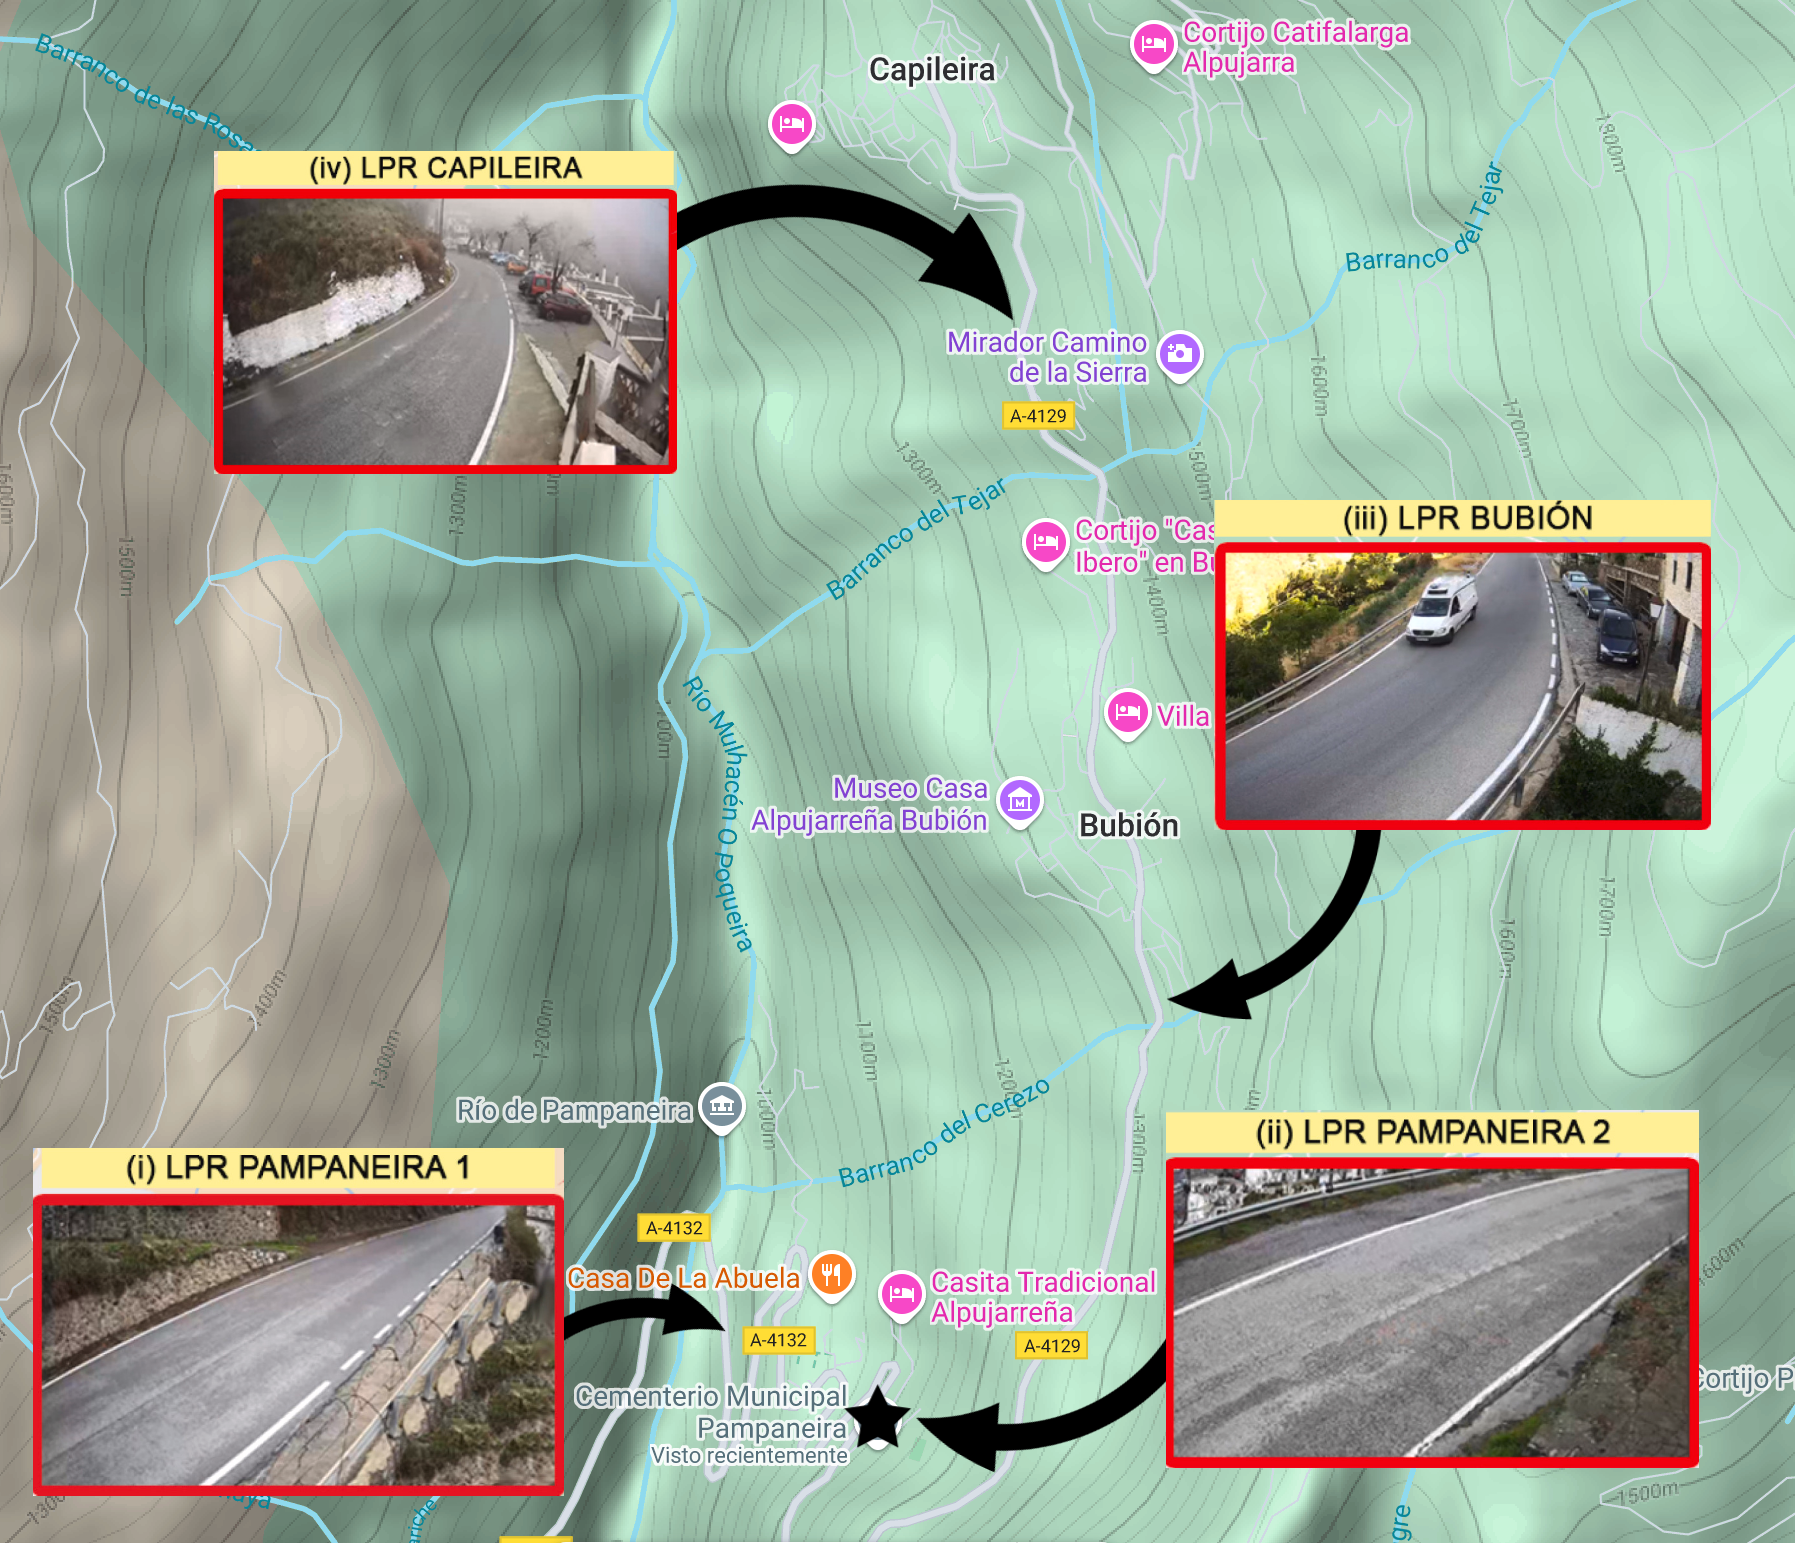
\includegraphics[width=0.53\textwidth]{images/mapa_fusion.png}
    \caption{Distribución geográfica de las cámaras \glsentryshort{lpr} en los municipios de Poqueira. Elaborada a partir de \citep{BolanosMartinez2024clustering}}
    \label{fig:mapa_fusion}
\end{figure}

La finalidad última es establecer las relaciones entre los patrones de tráfico vehicular y los niveles de contaminación atmosférica en esta región. Sin embargo, surge un desafío fundamental inherente a la naturaleza móvil de la unidad de medición de contaminantes: el camión de meteorología y contaminación opera en ubicaciones específicas (Pampaneira-Bubión) solo durante periodos de tiempo definidos:
\begin{itemize}
    \item \textbf{Capileira:} 16/11/2022 - 15/01/2023 (Estos datos no se tratan en este análisis específico de imputación por no estar el camión próximo a las ubicaciones de las cámaras.).
    \item \textbf{Pampaneira-Bubión (Cementerio):} 17/01/2023 - 14/03/2023.
    \item \textbf{Pampaneira-Bubión (Cementerio):} 06/06/2023 - 27/06/2023.
\end{itemize}

La operativa intrínsecamente discontinua de la unidad móvil, agravada por problemas prácticos como cortes de suministro eléctrico, robo de cableado, o el impacto de condiciones meteorológicas adversas (por ejemplo, lluvia de barro cegando las cámaras), además de fallos intermitentes de los sensores, genera \textbf{datos faltantes} significativos en las series temporales combinadas de tráfico y contaminación. Consecuentemente, la ausencia de estas mediciones impide un análisis continuo y completo de la relación tráfico-contaminación, lo que subraya la necesidad de abordar estos vacíos mediante técnicas de imputación.

Dada la presencia significativa de datos faltantes, un paso crucial antes de emprender análisis exhaustivos sobre la relación tráfico-contaminación es mejorar la calidad e integridad del dataset. Por ello, este trabajo se centra en la \textbf{aplicación y evaluación de diversas técnicas de imputación}. El propósito es reconstruir los valores ausentes de la manera más robusta y precisa posible, aprovechando la información contenida en los datos existentes. Al completar estas series temporales, se busca facilitar análisis posteriores más completos y, fundamentalmente, permitir el desarrollo de modelos predictivos o explicativos más fiables y con mayor poder inferencial.

\section{Conjuntos de Datos (Datasets)}
\label{sec:datasets}

Para llevar a cabo este estudio, se utilizan dos conjuntos de datos principales, derivados de la infraestructura IoT descrita.

\label{subsec:dataset_trafico}
El primer dataset consolida los registros agregados por hora del flujo vehicular detectado por las cuatro cámaras \glsentryshort{lpr} del proyecto Smart Poqueira, abarcando un periodo extenso desde febrero de 2022 hasta agosto de 2023. Cada fila del dataset representa una hora específica, y las columnas cuantifican el número de vehículos observados, categorizados según diversos criterios que se detallan a continuación. Este dataset proporciona una visión continua y detallada de la movilidad en la zona de estudio.

Las variables de este dataset se pueden agrupar en las siguientes categorías:

\begin{description}
    \item[\textbf{Identificación de Flujo por Cámara y Dirección (vehicles\_ID\_camera\_IN/OUT):}]
    Estas columnas cuantifican el número de vehículos detectados por una cámara específica y en una dirección determinada. El nombre de la columna sigue el patrón `vehicles\_IDCAM\_DIRECCION`.
        \begin{itemize}
            \item \texttt{IDCAM}: Identificador de la cámara \glsentryshort{lpr}. Puede tomar los siguientes valores:
                \begin{itemize}
                    \item \texttt{PAM\_1}: Cámara LPR 1 ubicada en Pampaneira.
                    \item \texttt{PAM\_2}: Cámara LPR 2 ubicada en Pampaneira (e.g., cerca del cementerio, cubriendo el acceso a Bubión).
                    \item \texttt{BUB}: Cámara LPR ubicada en Bubión.
                    \item \texttt{CAP}: Cámara LPR ubicada en Capileira.
                \end{itemize}
            \item \texttt{DIRECCION}: Indica el sentido del flujo vehicular. Puede ser:
                \begin{itemize}
                    \item \texttt{IN}: Vehículos entrando al núcleo urbano o zona monitorizada por la cámara.
                    \item \texttt{OUT}: Vehículos saliendo del núcleo urbano o zona monitorizada por la cámara.
                \end{itemize}
            \textit{Ejemplo: La columna \texttt{vehicles\_PAM\_1\_IN} contabiliza el número de vehículos que entraron por la cámara PAM\_1 durante esa hora.}
        \end{itemize}

    \item[\textbf{Origen Geográfico del Vehículo (Zona\_...):}]
    Estas columnas agrupan los vehículos según la provincia o comunidad autónoma de origen de su matrícula a partir de los datos de la Dirección General de Tráfico (DGT).
        \begin{itemize}
            \item \texttt{Zona\_Catalunia\_y\_Otras}: Vehículos procedentes de Cataluña, La Rioja, Aragón, Illes Balears, Euskadi, Navarra, Galicia, Asturias, Cantabria, o Castilla y León.
            \item \texttt{Zona\_Comunidad\_de\_Madrid}: Vehículos procedentes de la Comunidad de Madrid.
            \item \texttt{Zona\_Andalucia\_no\_GR}: Vehículos procedentes de las provincias de Andalucía, excluyendo Granada (i.e., Almería, Cádiz, Córdoba, Huelva, Jaén, Málaga, Sevilla).
            \item \texttt{Zona\_Granada}: Vehículos procedentes de la provincia de Granada.
            \item \texttt{Zona\_Extremadura\_y\_Otras}: Vehículos procedentes de Extremadura, Castilla-La Mancha, Región de Murcia, Comunitat Valenciana, Canarias, Ceuta o Melilla.
        \end{itemize}

    \item[\textbf{Características del Vehículo: Emisiones de CO2 (co2\_intervalo\_...):}]
    Estas columnas clasifican los vehículos según el intervalo de emisiones de CO2 (en g/km) asociado a su modelo, obtenido a partir de la información de la DGT.
        \begin{itemize}
            \item \texttt{co2\_0-100}: Vehículos con emisiones de CO2 menores o iguales a 100 g/km.
            \item \texttt{co2\_101-200}: Vehículos con emisiones de CO2 entre 101 y 200 g/km (ambos inclusive).
            \item \texttt{co2\_201-300}: Vehículos con emisiones de CO2 entre 201 y 300 g/km (ambos inclusive).
            \item \texttt{co2\_+300}: Vehículos con emisiones de CO2 superiores a 300 g/km.
        \end{itemize}

    \item[\textbf{Características del Vehículo: Número de Asientos (seats\_...):}]
    Clasificación de los vehículos según el número de asientos.
        \begin{itemize}
            \item \texttt{seats\_5\_seats}: Vehículos con exactamente 5 asientos.
            \item \texttt{seats\_+5\_seats}: Vehículos con más de 5 asientos.
            \item \texttt{seats\_-5\_seats}: Vehículos con menos de 5 asientos.
        \end{itemize}

    \item[\textbf{Características el Vehículo: Etiqueta Ambiental DGT (label\_...):}]
    Categorización de los vehículos según la etiqueta ambiental oficial de la DGT.
        \begin{itemize}
            \item \texttt{label\_Sin\_Etiqueta}: Vehículos que no disponen de etiqueta ambiental (generalmente los más antiguos y contaminantes).
            \item \texttt{label\_C}: Vehículos con etiqueta ambiental C.
            \item \texttt{label\_B}: Vehículos con etiqueta ambiental B.
            \item \texttt{label\_ECO}: Vehículos con etiqueta ambiental ECO.
            \item \texttt{label\_0}: Vehículos con etiqueta ambiental Cero Emisiones (0).
        \end{itemize}
        \textit{Nota: Esta información se obtiene mediante técnicas de web scraping de fuentes oficiales de la DGT a partir de la matrícula.}

\end{description}

\subsection*{Dataset de Intersección Tráfico-Contaminación}
\label{subsec:dataset_contaminacion}
El segundo dataset fusiona temporalmente los datos de tráfico con las mediciones del camión móvil, conteniendo únicamente registros horarios de los períodos y ubicaciones donde el camión estuvo operativo en Pampaneira/Bubión. Es un subconjunto temporal del dataset de tráfico, enriquecido con variables ambientales. Estas variables de contaminación son: 

\begin{description}
    \item[\textbf{\texttt{\MakeTextUppercase{co}}}] \textbf{Monóxido de Carbono:} Concentración media horaria medida con el analizador Thermo Scientific mod. 48i. Es un trazador de combustión incompleta, que principalmente procede de vehículos de gasolina en condiciones de arranque en frío o ralentí, y también de la quema de biomasa. Unidades: miligramos por metro cúbico (mg/m³).

    \item[\textbf{\texttt{\MakeUppercase{no}}}] \textbf{Monóxido de Nitrógeno:} Concentración media horaria medida con el analizador Thermo Scientific mod. 42i. Es un contaminante primario emitido directamente por procesos de combustión a alta temperatura, siendo un \textbf{trazador importante del tráfico diésel}. Unidades: microgramos por metro cúbico (µg/m³).

    \item[\textbf{\texttt{\MakeUppercase{no2}}}] \textbf{Dióxido de Nitrógeno:} Concentración media horaria medida con el analizador Thermo Scientific mod. 42i. Se forma principalmente por la oxidación del NO en la atmósfera, aunque también se emite directamente por los coches aunque en menor medida. Es, junto con el NO, un \textbf{trazador clave del tráfico diésel} y otros procesos de combustión. Unidades: microgramos por metro cúbico (µg/m³).

    \item[\textbf{\texttt{\MakeUppercase{o3}}}] \textbf{Ozono Troposférico:} Concentración media horaria medida con el analizador Thermo Scientific mod. 49i. Es un contaminante secundario, no emitido directamente, sino formado en la atmósfera por reacciones fotoquímicas entre óxidos de nitrógeno (NOx) y compuestos orgánicos volátiles (COVs) en presencia de luz solar. Unidades: microgramos por metro cúbico (µg/m³).

    \item[\textbf{\texttt{\MakeUppercase{so2}}}] \textbf{Dióxido de Azufre:} Concentración media horaria medida con el analizador Thermo Scientific mod. 43i. Proviene principalmente de la combustión de combustibles fósiles que contienen azufre (carbón, fuelóleo). Su relevancia como trazador del tráfico rodado actual es limitada debido a las bajas concentraciones de azufre en gasolinas y gasóleos modernos. Unidades: microgramos por metro cúbico (µg/m³).

    \item[\textbf{\texttt{\MakeUppercase{pm10}}}] \textbf{Material Particulado < 10 µm:} Concentración media horaria de partículas en suspensión con un diámetro aerodinámico inferior a 10 micrómetros, obtenida con el Monitor TEOM 1405 (Thermo Scientific). Incluye una mezcla compleja de partículas de diversas fuentes: combustión (tráfico, industria, calefacción), polvo en suspensión, aerosoles secundarios, fuentes naturales, etc. Unidades: microgramos por metro cúbico (µg/m³).

    \item[\textbf{\texttt{eBC\_tot}}] \textbf{Carbono Negro Total (Hollín):} Concentración media horaria de carbono negro total obtenida con el fotómetro de absorción Aethalometer AE31. El carbono negro es un producto de la combustión incompleta de material carbonoso y es un componente importante del material particulado fino. Unidades: microgramos por metro cúbico (µg/m³).

    \item[\textbf{\texttt{eBC\_ff}}] \textbf{Carbono Negro de Combustibles Fósiles:} Concentración media horaria de carbono negro atribuible específicamente a la combustión de combustibles fósiles (gasolina, diésel). Se obtiene aplicando el modelo del etalómetro \citep{sandradewi_source_2008}. Es considerado un \textbf{trazador primario y específico del tráfico vehicular}. Unidades: microgramos por metro cúbico (µg/m³).

    \item[\textbf{\texttt{eBC\_bb}}] \textbf{Carbono Negro de Quema de Biomasa:} Concentración media horaria de carbono negro atribuible específicamente a la quema de biomasa (leña para calefacción, quemas agrícolas, incendios forestales). Se obtiene aplicando el modelo del etalómetro  \citep{sandradewi_source_2008}. Unidades: microgramos por metro cúbico (µg/m³).
\end{description}

\subsubsection*{Variables Meteorológicas}
\begin{description}
    \item[\textbf{\texttt{TEMP}}] \textbf{Temperatura del Aire:} Temperatura media horaria (°C) medida por el transmisor YOUNG 92000 ResponseONE. Afecta las tasas de reacción química atmosférica. Temperaturas invernales anómalamente elevadas pueden indicar la presencia de inversiones térmicas asociadas a condiciones anticiclónicas. Estas inversiones limitan la dispersión vertical y favorecen la acumulación de contaminantes en superficie, pudiendo generar episodios de alta contaminación \citep{Wallace2006atmospheric, Seinfeld2016atmospheric}.

    \item[\textbf{\texttt{RH}}] \textbf{Humedad Relativa:} Humedad relativa media horaria del aire medida por el transmisor YOUNG 92000. Afecta a la formación de aerosoles secundarios, la visibilidad y puede influir en la deposición de contaminantes. Alta humedad puede correlacionarse con condiciones de estancamiento o niebla. Unidades: porcentaje (\%).

    \item[\textbf{\texttt{WS}}] \textbf{Velocidad del Viento:} Velocidad media horaria del viento medida por el anemómetro de la torre meteorológica. Es un factor fundamental para la dispersión horizontal de los contaminantes; velocidades bajas favorecen la acumulación. Unidades: metros por segundo (m/s).

    \item[\textbf{\texttt{WD}}] \textbf{Dirección del Viento:} Dirección media horaria desde la que sopla el viento, medida en la torre meteorológica. 0° corresponde al Norte geográfico. Es crucial para identificar el transporte de contaminantes desde posibles áreas fuente. Unidades: grados (°).

    \item[\textbf{\texttt{PRES}}] \textbf{Presión Atmosférica:} Presión atmosférica media horaria a nivel de la estación de medición. Altas presiones suelen asociarse con condiciones meteorológicas estables (anticiclones) que, combinadas con vientos bajos, dificultan la dispersión vertical y horizontal de los contaminantes, favoreciendo episodios de alta contaminación. Unidades: hectopascales (hPa).
\end{description}


\begin{description}
    \item[\textbf{\texttt{truck\_pos}}] \textbf{Posición del Camión Meteorológico:} Variable categórica que indica la cámara \glsentryshort{lpr} más cercana a la ubicación física del camión de medición durante la hora correspondiente. Los valores posibles en este dataset son \texttt{'CAP'} (cuando estaba en Capileira) y \texttt{'PAM\_2'} (cuando estaba en la ubicación del cementerio de Pampaneira, monitorizado por la cámara PAM\_2). Esta variable permite asociar las mediciones de contaminación con el flujo de tráfico específico de la cámara más próxima.
\end{description}

En la Figura ~\ref{fig:truck_pos_dist} se puede observar los registros para cada localización distinta del camión.

\begin{figure}[htbp]
    \centering
    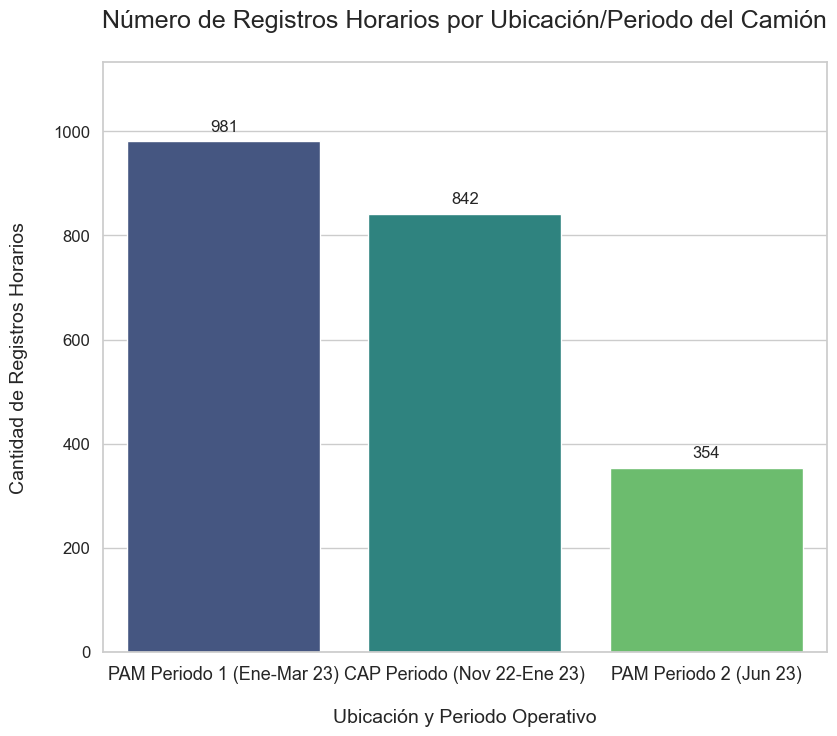
\includegraphics[width=0.6\textwidth]{images/EDA/truck_pos.png}
    \caption{Distribución del número de registros horarios en el dataset de intersección (\texttt{trafico\_contamina\_interseccion}) según la ubicación y periodo operativo del camión móvil de medición}
    \label{fig:truck_pos_dist}
\end{figure}

Este dataset hereda también las columnas de tráfico vehicular correspondientes a la hora y cámara más cercana. Es el dataset principal para el análisis y la imputación.

\section{Análisis Exploratorio de Datos (EDA)}
\label{sec:eda}

Se efectuó un Análisis Exploratorio de Datos (EDA) sobre el dataset de trafico-intersección para comprender las distribuciones, identificar patrones, valores atípicos, datos faltantes y correlaciones.

Se realizó un análisis de valores faltantes, distribución de variables y análisis de correlaciones.

\subsection{Análisis del Porcentaje de Valores Faltantes}


\textbf{Análisis de la Figura ~\ref{fig:porcentajes_nulos}:}
En este periodo, las variables con la mayor proporción de valores faltantes son \textbf{WS} (Velocidad del Viento) y \textbf{WD} (Dirección del Viento), ambas con un \textbf{60.6\%} de datos ausentes. Les siguen notablemente \textbf{eBC\_ff} y \textbf{eBC\_bb}, cada una con un \textbf{43.7\%} de valores faltantes. \textbf{PM10} presenta un \textbf{30.9\%} de ausencia, mientras que \textbf{O3}, \textbf{NO2}, \textbf{NO} y \textbf{CO} muestran porcentajes de valores faltantes aproximados al \textbf{27-28\%}. El resto de las variables de tráfico (como \texttt{vehicles\_PAM\_1\_OUT}, \texttt{vehicles\_PAM\_1\_OUT\_Zona\_Granada}, etc.) también se sitúan alrededor del \textbf{27.3\%} de datos faltantes.

\textbf{Análisis de la Figura ~\ref{fig:porcentajes_nulos2}:}
En contraste con el Periodo 1, la variable \textbf{PM10} se destaca como la de mayor incidencia de datos faltantes en este periodo, alcanzando un notable \textbf{80.2\%}. Las variables \textbf{WS} y \textbf{WD} ahora presentan un \textbf{30.8\%} de ausencia, seguidas de cerca por \textbf{eBC\_ff} y \textbf{eBC\_bb} con \textbf{29.2\%}. Las variables de contaminación \textbf{CO}, \textbf{NO2}, \textbf{NO} y \textbf{O3} muestran porcentajes muy similares, alrededor del \textbf{28.3\%}. Las variables de tráfico también mantienen un nivel constante de datos faltantes, aproximadamente el \textbf{28.1\%}.

%En concreto, se observa, en la Figura ~\ref{fig:porcentajes_nulos}, la mayor incidencia en \texttt{eBC\_tot} (69.3\%), seguida por \texttt{eBC} (49.5\%) y \texttt{SO2} (48.8\%). Variables como \texttt{WS}, \texttt{WD}, y \texttt{PM10} también presentan una notable proporción de datos ausentes superior al 20\%.

\begin{figure}[htbp]
    \centering
    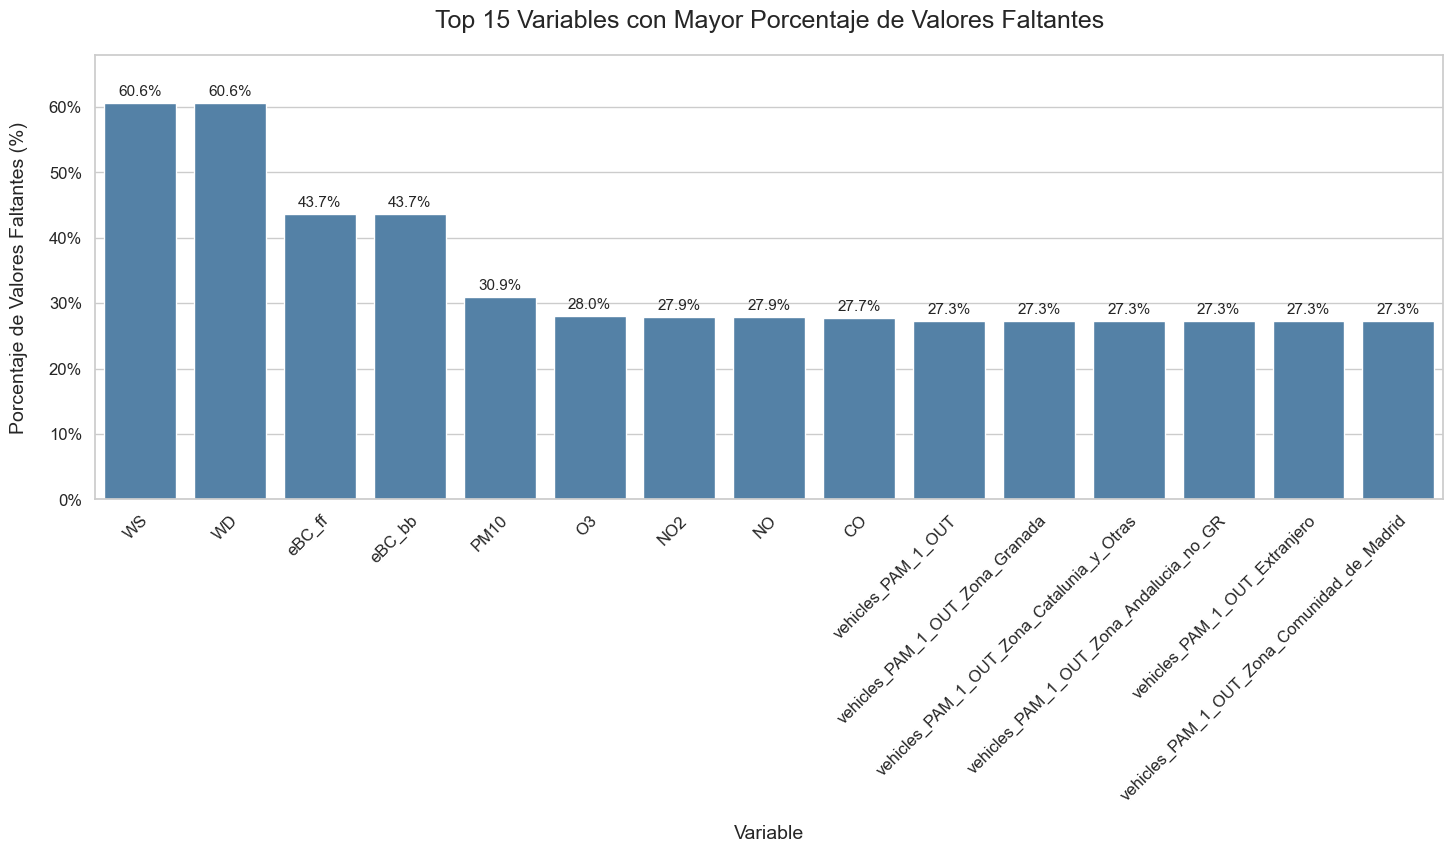
\includegraphics[width=0.9\textwidth]{images/EDA/porcentajes_per1.png} 
    \caption{Porcentaje de valores faltantes para las 15 variables con mayor proporción de ausencias en el Periodo 1.}
    \label{fig:porcentajes_nulos}
\end{figure}

\begin{figure}[htbp]
    \centering
    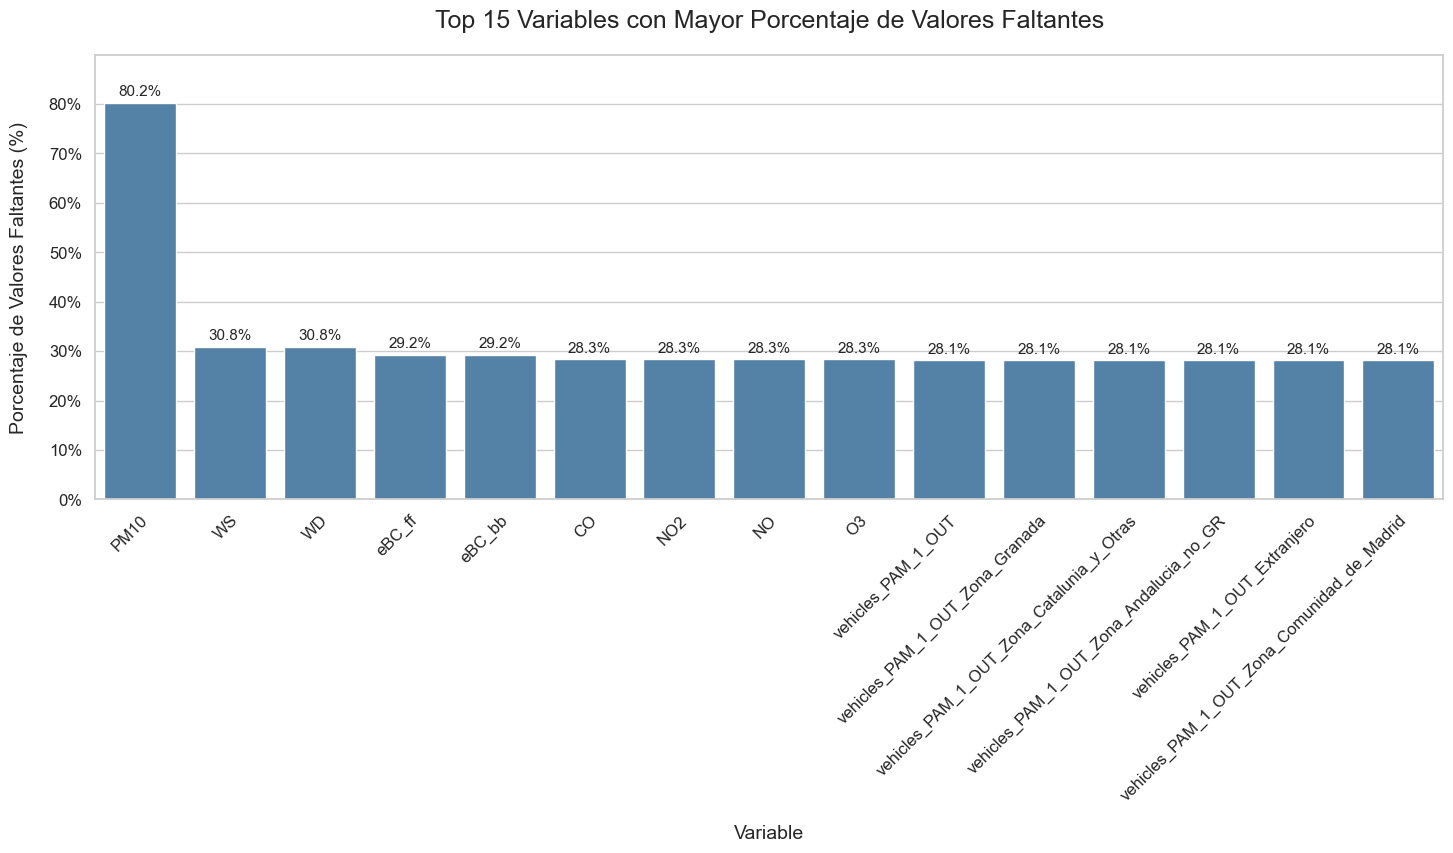
\includegraphics[width=0.9\textwidth]{images/EDA/porcentajes_per2.png} 
    \caption{Porcentaje de valores faltantes para las 15 variables con mayor proporción de ausencias en el Periodo 2}
    \label{fig:porcentajes_nulos2}
\end{figure}

\clearpage

%\begin{itemize}
    Los histogramas de los \textbf{contaminantes (CO, NO, NO2):}  (Figura~\ref{fig:hist_co}) mostraron distribuciones con fuerte asimetría derecha, indicando predominio de concentraciones bajas con picos ocasionales altos, característico de fuentes como el tráfico.

    \begin{figure}[htbp]
        \centering
        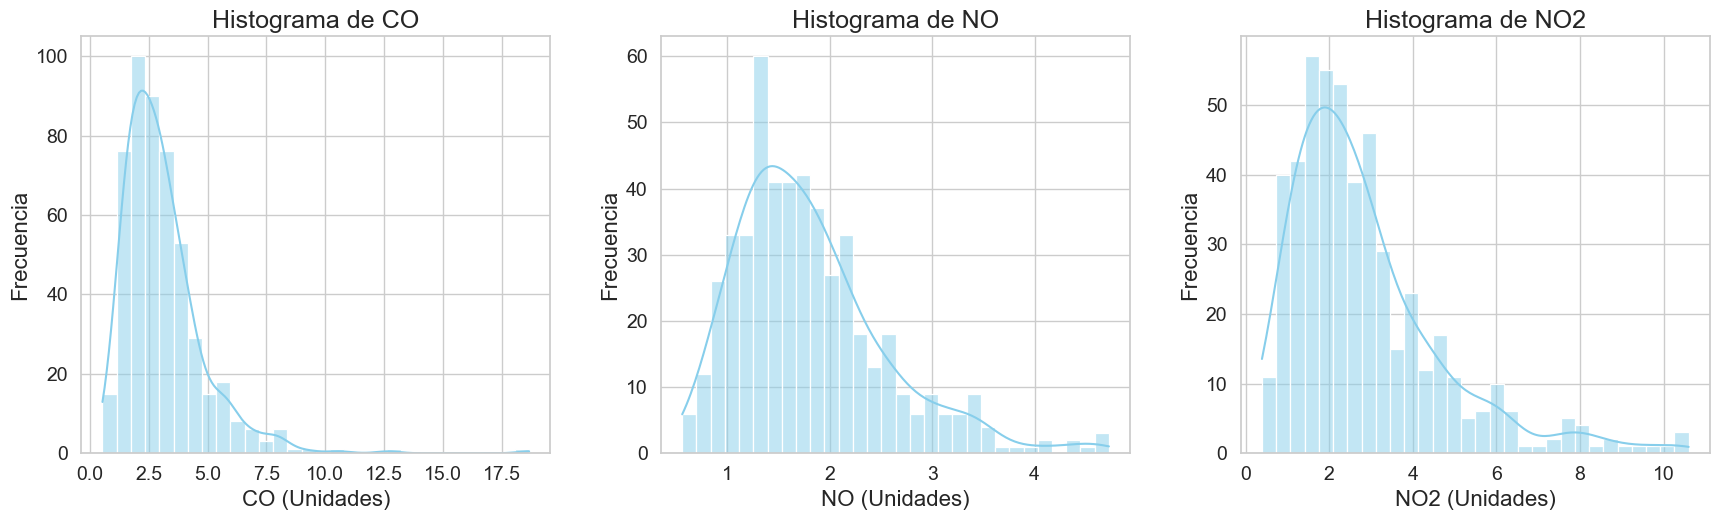
\includegraphics[width=\textwidth]{images/EDA/histogramas_co.png}
        \caption{Histogramas de las concentraciones horarias de CO, NO y NO2. Se observa una clara asimetría hacia la derecha en las tres distribuciones.}
        \label{fig:hist_co}
    \end{figure}

    Los diagramas de caja de los \textbf{contaminantes (O3, SO2, PM10, eBC):}  (Figura ~\ref{fig:diagrama_cajas}) revelaron valores atípicos, especialmente en \texttt{O3} y \texttt{PM10}. La mediana de \texttt{SO2} fue muy baja. Las fracciones de \texttt{eBC} mostraron diferencias en sus rangos y medianas.

    % --- LaTeX Code to Insert the Combined Image ---

    \begin{figure}[htbp] 
    \centering 

    % Otras opciones son: 0.8\textwidth, 10cm, etc.
    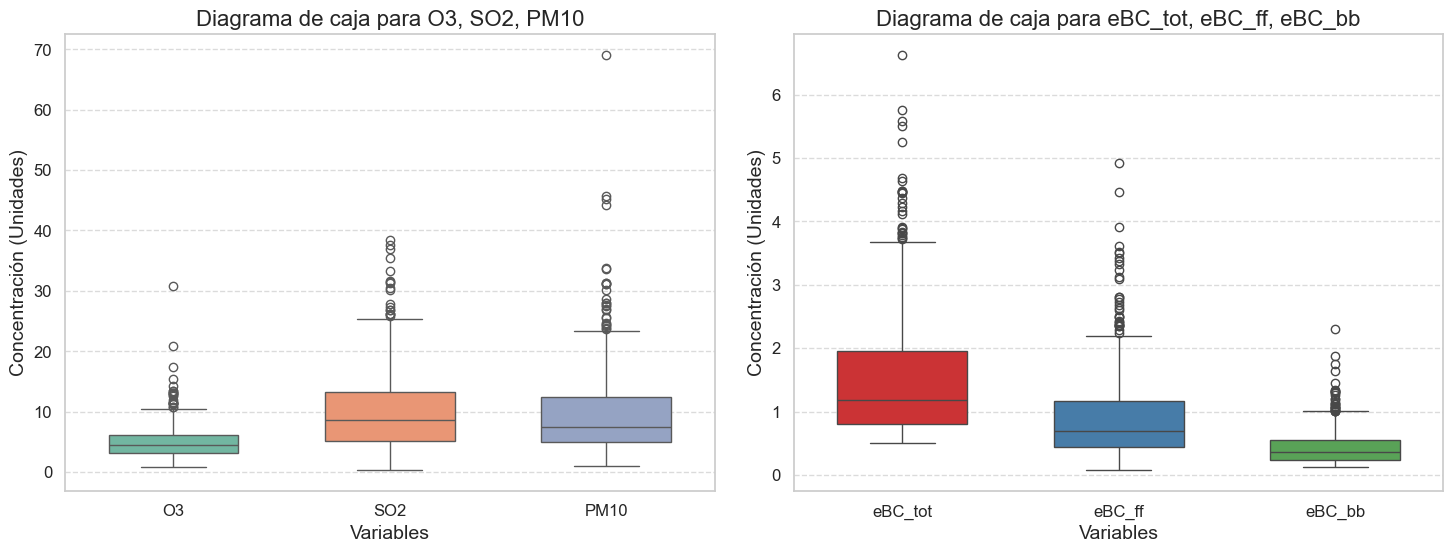
\includegraphics[width=0.9\linewidth]{images/EDA/diagrama_cajas.png}

    \caption{Diagramas de caja comparativos para variables de contaminación. A la izquierda se muestran O3, SO2 y PM10. A la derecha se muestran las variables relacionadas con el carbono negro elemental (eBC\_tot, eBC\_ff, eBC\_bb).}

    \label{fig:diagrama_cajas}

    \end{figure}

    \clearpage

    Los histogramas de \textbf{meteorología (TEMP, RH, WS):}  (Figura~\ref{fig:hist_temp}) mostraron distribuciones más variadas: \texttt{TEMP} bimodal (ciclos día/noche), \texttt{RH} más centrada, y \texttt{WS} con fuerte asimetría derecha (predominio de vientos bajos).

    \begin{figure}[htbp]
        \centering
        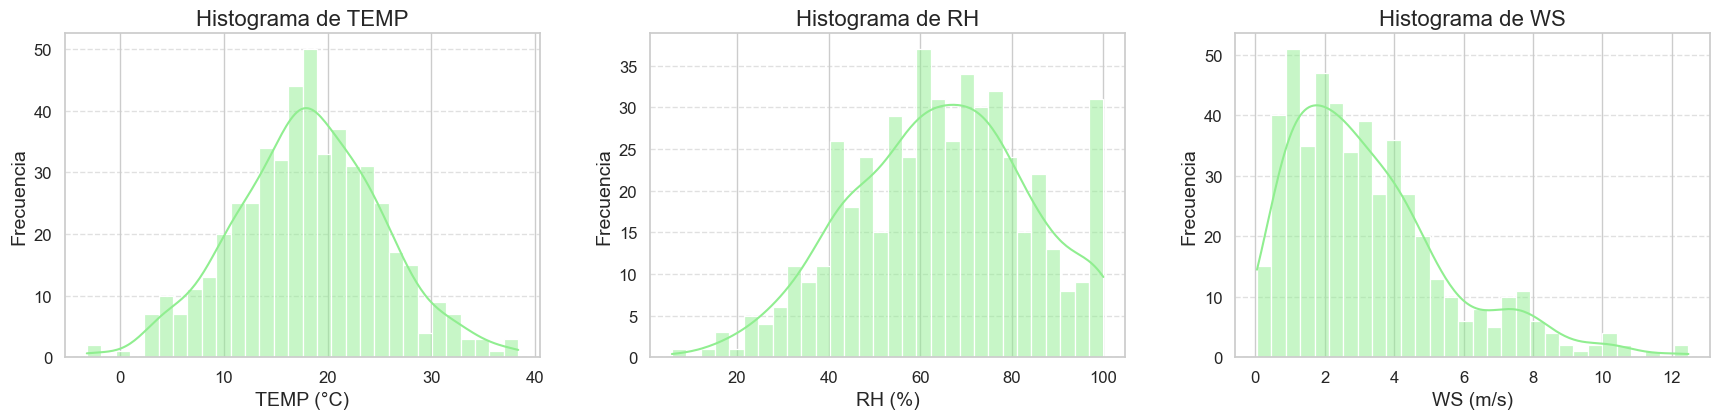
\includegraphics[width=\textwidth]{images/EDA/histogramas_3.png}
        \caption{Histogramas de las variables meteorológicas TEMP (Temperatura), RH (Humedad Relativa) y WS (Velocidad del Viento).}
        \label{fig:hist_temp}
    \end{figure}

%\end{itemize}

\label{subsec:correlaciones}
La matriz de correlación (Figura~\ref{fig:matriz_corr}) mostró relaciones significativas:
\begin{itemize}
    \item \textbf{Positivas Fuertes:} \texttt{eBC\_tot} con \texttt{eBC\_ff} (0.76) y \texttt{eBC\_bb} (0.64); \texttt{NO2} con \texttt{eBC\_tot} (0.69); \texttt{NO} con \texttt{NO2} (0.64); \texttt{O3} con \texttt{TEMP} (~0.4).
    \item \textbf{Negativas Moderadas:} \texttt{RH} con \texttt{O3} (~-0.5); \texttt{RH} con \texttt{TEMP} (~-0.5).
    \item \textbf{Otras:} Correlaciones negativas débiles entre contaminantes primarios (NOx, eBC) y O3. Correlaciones débiles entre meteorología y contaminantes primarios.
\end{itemize}
Estas correlaciones, especialmente las ligadas a trazadores de tráfico, son clave para la imputación basada en modelos predictivos.

\begin{figure}[H] % Forzar la ubicación aquí
    \centering
    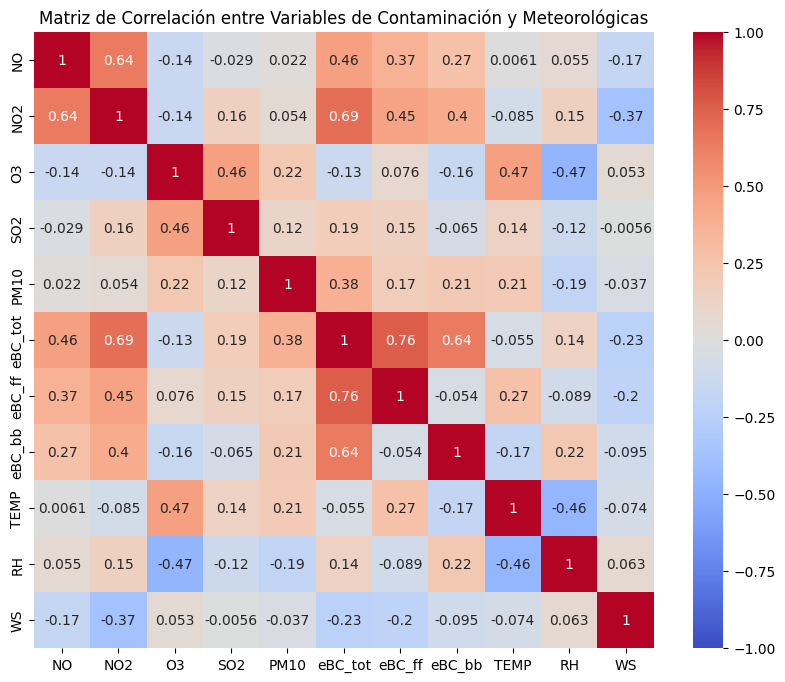
\includegraphics[width=0.5\textwidth, angle=0]{images/EDA/matriz_correlacion.png} % Puedes ajustar el ángulo si es necesario
    \caption{Matriz de correlación de Pearson entre las principales variables de contaminación}
    \label{fig:matriz_corr}
\end{figure}

\section{Entorno Experimental y Flujo de Trabajo}
\label{sec:desarrollo_entorno}
Para llevar a cabo la parte práctica de este trabajo, centrada en la imputación de datos faltantes en series temporales de contaminación atmosférica, se ha desarrollado una solución específica mediante la creación de un paquete de Python denominado \texttt{pampaneira\_imputation} \footnote{\url{https://github.com/eigenric/TFG/tree/main/pampaneira_imputation}}. Este paquete organiza de forma modular toda la lógica necesaria para el preprocesamiento de datos, la aplicación de los diversos métodos de imputación seleccionados y la evaluación sistemática de sus resultados.

\subsection{Estructura del Paquete \texttt{pampaneira\_imputation}}
El paquete \texttt{pampaneira\_imputation} ha sido estructurado en varios módulos, cada uno con responsabilidades bien definidas para facilitar el mantenimiento, la escalabilidad y la claridad del código. La estructura principal del paquete es la siguiente:
\begin{itemize}
    \item \textbf{\texttt{\_\_init\_\_.py}}: Archivo estándar que permite que el directorio sea tratado como un paquete de Python.
    \item \textbf{\texttt{config.py}}: Centraliza todos los parámetros de configuración globales del proyecto. Esto incluye rutas de archivos de datos, fechas de inicio y fin de los periodos de estudio, hiperparámetros de los modelos de aprendizaje profundo, nombres de las columnas de características, entre otros. Esta centralización facilita la modificación de parámetros para diferentes ejecuciones y experimentos.
    \item \textbf{\texttt{data\_loader.py}}: Contiene las funciones responsables de cargar los conjuntos de datos originales desde sus fuentes (e.g., archivos CSV). Este módulo también puede realizar una limpieza inicial o transformaciones básicas que sean comunes a todos los datos antes del preprocesamiento específico para la imputación.
    \item \textbf{\texttt{data\_preprocessor.py}}: Implementa toda la lógica para el preprocesamiento de los datos. Sus funciones se encargan de la división de los datos en conjuntos de entrenamiento, validación y prueba según los periodos definidos; el escalado de las características numéricas (e.g., mediante \texttt{StandardScaler}); la creación de ventanas temporales o secuencias para los modelos que las requieran; y, crucialmente, la eliminación artificial de datos en los conjuntos de validación y prueba para permitir una evaluación controlada de los métodos de imputación.
    \item \textbf{\texttt{evaluation.py}}: Define las funciones para calcular las métricas de rendimiento (RMSE, MSE, MAE, MRE) que se utilizan para evaluar la precisión y la calidad de las imputaciones realizadas por los diferentes métodos.
    \item \textbf{\texttt{imputation\_methods.py}}: Este módulo es el núcleo del proyecto donde se agrupan las implementaciones de los diferentes algoritmos de imputación evaluados. Incluye tanto métodos simples (media, mediana, interpolación lineal, forward fill, backward fill) como los modelos más avanzados basados en aprendizaje profundo (Transformer, SAITS). Para estos últimos, parte de la funcionalidad se ha construido aprovechando las capacidades de la librería \textbf{PyPOTS} \citep{du2023pypots}, una biblioteca especializada en el procesamiento de datos con patrones irregulares y datos faltantes en series temporales.
    \item \textbf{\texttt{utils.py}}: Recopila un conjunto de funciones auxiliares de propósito general que son utilizadas a lo largo de todo el paquete. Ejemplos de estas utilidades pueden ser funciones para la creación de ventanas deslizantes a partir de secuencias, la eliminación artificial de datos con patrones específicos, o el reformateo de estructuras de datos.
\end{itemize}

\subsection{Flujo de Trabajo y Experimentación}
El flujo de trabajo principal (pipeline) para la ejecución de los experimentos y la obtención de los resultados comparativos entre los métodos de imputación se ha orquestado y documentado mediante un Jupyter Notebook principal, denominado \texttt{Notebook\_Imputation.ipynb}. Este notebook guía al usuario o investigador a través de los siguientes pasos metodológicos:
\begin{enumerate}
    \item \textbf{Configuración Inicial:} Carga de los parámetros del proyecto definidos en el módulo \texttt{config.py}.
    \item \textbf{Carga de Datos:} Adquisición de los datos crudos de contaminación y meteorológicos utilizando las funciones provistas por \texttt{data\_loader.py}.
    \item \textbf{Preprocesamiento:} Aplicación de las rutinas de preprocesamiento de \texttt{data\_preprocessor.py}, que incluyen la segmentación temporal, el escalado de características, la generación de secuencias apropiadas para los modelos y la eliminación controlada de datos en los subconjuntos designados para la evaluación.
    \item \textbf{Aplicación de Métodos de Imputación:} Ejecución secuencial de los diferentes métodos de imputación definidos en \texttt{imputation\_methods.py} sobre los datos preprocesados con datos eliminados artificialmente. Para los modelos de aprendizaje profundo, esto incluye la carga de modelos pre-entrenados o su entrenamiento si es la primera ejecución o si se han modificado los parámetros.
    \item \textbf{Evaluación Cuantitativa:} Cálculo del rendimiento de cada método de imputación utilizando el conjunto de métricas implementadas en \texttt{evaluation.py}. Esta evaluación se realiza comparando los valores imputados con los valores originales verdaderos únicamente en las posiciones donde se eliminaron datos artificialmente.
    \item \textbf{Análisis y Visualización de Resultados:} Presentación tabular de las métricas de error y generación de visualizaciones (como las series temporales comparativas) para un análisis cualitativo del comportamiento de los métodos.
\end{enumerate}
Este enfoque estructurado mediante un notebook facilita la reproducibilidad de los experimentos y proporciona una documentación clara del proceso seguido para la obtención de los resultados.

\subsection{Control de Versiones y Pruebas Unitarias}
El desarrollo íntegro del código fuente del paquete \texttt{pampaneira\_imputation}, así como del \textbf{Jupyter Notebook\footnote{\url{https://github.com/eigenric/TFG/blob/main/notebooks/Notebook_Imputation.ipynb}}} de experimentación, se ha gestionado mediante el sistema de control de versiones Git. El repositorio que contiene todo el código fuente, los datos (o enlaces a ellos) y los materiales complementarios del proyecto se encuentra disponible públicamente en la plataforma GitHub.

Adicionalmente, con el fin de asegurar la correcta funcionalidad y la fiabilidad de los componentes clave del paquete de software desarrollado, se ha implementado una serie de \textbf{pruebas unitarias}. Estos tests automatizados verifican el comportamiento esperado de funciones críticas, particularmente aquellas involucradas en el preprocesamiento de los datos (como la creación de ventanas o la introducción de datos faltantes) y en el cálculo de las métricas de evaluación. La inclusión de pruebas unitarias contribuye significativamente a la robustez del código, facilita la detección temprana de errores durante el desarrollo y permite realizar refactorizaciones con mayor confianza.


\section{Preparación de Datos y Configuración Experimental}
\label{sec:data_prep_setup_revised}

El proceso se inicia con los datos crudos de series temporales multivariantes de Pampaneira-Bubión. Recordemos que el camión y la cámara PAM\_2 se encuentran ubicados en el cementerio municipal de Pampaneira. Tratamos, por proximidad, los datos de Pampaneira y Bubión y descartamos Capileira.

\subsection{Carga, Estructura y Preprocesamiento Inicial}
\label{subsec:load_preprocess_revised}
Los datos originales, que pueden contener faltantes naturales, son cargados utilizando rutinas del módulo \texttt{pampaneira\_imputation.data\_loader}. 
A continuación, para garantizar una estructura de serie temporal multivariante completa y regular, una función del módulo \texttt{pampaneira\_imputation.data\_preprocessor} completa el índice temporal horario para los periodos de estudio. Si originalmente faltan registros para ciertas horas, se insertan filas nuevas para esos instantes, rellenando todas las características con valores NaN, asegurando así la continuidad requerida para los análisis posteriores. 
Los datos se organizan en una estructura tensorial 3D $(N \times T \times D)$, donde $N$ es el número de muestras (ventanas temporales), $T=24$ es la longitud fija de la ventana, y $D$ el número de características. El valor $T=24 horas$ se ha elegido para poder seguir los patrones diarios de vehículos y ambientales. Los datos se dividen por periodos temporales para análisis separados.

\subsection{División, Escalado y Creación del Escenario de Evaluación}
\label{subsec:split_scale_eval_setup}
El núcleo del preprocesamiento, gestionado por el módulo \\ \texttt{pampaneira\_imputation.data\_preprocessor}, aplica los siguientes pasos a los datos de cada periodo:
\begin{enumerate}
    \item \textbf{División Train/Validation/Test:} Segmentación cronológica de los datos en conjuntos de entrenamiento (80\%), validación (20\% del de entrenamiento) y prueba (20\% final), según las duraciones especificadas.
    \item \textbf{Escalado (Normalización Z-score):} Aplicación de escalado estándar a las características seleccionadas, ajustando el escalador (\textit{fitting}) solo sobre el conjunto de entrenamiento y aplicándolo (\textit{transforming}) a los tres conjuntos.
    Para una característica $j$ en el dataset, su valor estandarizado $x'_{ij}$ para la $i$-ésima muestra se calcula como:
    \begin{equation}
    x'_{ij} = \frac{x_{ij} - \mu_j}{\sigma_j}
    \label{eq:zscore}
    \end{equation}
    donde $x_{ij}$ es el valor original de la característica $j$ para la muestra $i$, $\mu_j$ es la media de la característica $j$, y $\sigma_j$ es la desviación estándar de la característica $j$.
    Es crucial que los parámetros del escalador (la media $\mu_j$ y la desviación estándar $\sigma_j$ para cada característica) se calculen (\textit{fitting}) \textbf{únicamente} sobre el conjunto de entrenamiento. Posteriormente, esta transformación (con los parámetros aprendidos del entrenamiento) se aplica (\textit{transforming}) a los tres conjuntos: entrenamiento, validación y prueba. Este procedimiento evita la fuga de información (data leakage) del conjunto de prueba al de entrenamiento, asegurando una evaluación más realista del rendimiento del modelo.
    \item \textbf{Ventaneo (Windowing):} Creación de secuencias de longitud $T=24$ mediante una ventana deslizante, resultando en la estructura tensorial 3D $(N \times T \times D)$.
    \item \textbf{Eliminación de datos para crearlos artificialmente:} Se eliminan artificialmente un 10\% de los valores previamente observados (después de escalar y ventanear) en cada split (train, val, test), siguiendo un patrón configurado. En este estudio, se consideran tres patrones para simular diferentes tipos de ausencia de datos:
\begin{itemize}
\item \textbf{'point' (Puntual):} Introduce valores NaN de forma aleatoria e independiente en cualquier posición del tensor de datos, simulando fallos esporádicos. Este es el patrón que utilizamos por defecto.
\item \textbf{'subseq' (Ráfaga):} Genera huecos o ráfagas de valores NaN de longitud variable en posiciones aleatorias dentro de cada serie temporal individual (por característica y muestra), simulando interrupciones temporales de sensores.
\item \textbf{'block' (Bloque desde el inicio):} Crea bloques de NaN de longitud variable que comienzan siempre desde el inicio de la secuencia temporal (por característica y muestra), simulando, por ejemplo, datos ausentes al comienzo de un periodo de medición.
\end{itemize}
Este paso es crucial para poder comprobar la fiabilidad de los modelos de reconstrucción de la señal.
\end{enumerate}


Esta fase de preprocesamiento define formalmente los siguientes conjuntos de datos y máscaras utilizados en el experimento:

\begin{itemize}
    \item \textbf{$\mathcal{X}_{\text{orig}}$}: El tensor de datos escalados y ventaneados (windowing) \textit{antes} de eliminar los faltantes artificiales. Este tensor carece de los faltantes naturales originales, pero no de los artificiales y sirve como verdad absoluta o \textbf{ground truth} para la evaluación.
    \item \textbf{$\mathbf{M}_{\text{natural}}$}: La máscara binaria que indica la posición de los faltantes naturales en $\mathcal{X}_{\text{orig}}$ ($0=$faltante, $1=$observado).
    \item \textbf{$\mathbf{M}_{\text{artificial}}$}: La máscara binaria que indica las posiciones donde se eliminaron faltantes \textit{artificialmente} ($1=$eliminado artificialmente, $0=$no eliminado).
    \item \textbf{$\mathcal{X}_{\text{missing}}$}: El tensor de datos utilizado como \textbf{entrada} para los métodos de imputación. Le faltan tanto los naturales como los artificiales.

    
\end{itemize}

\textbf{La imputación se realiza sobre \textbf{$\mathcal{X}_{\text{missing}}$}, pero la evaluación de la precisión se centra exclusivamente en la capacidad de los modelos para recuperar estos valores faltantes eliminados artificialmente \textbf{$M_{artificial}$}, ya que para ellos se conoce el valor verdadero original (`ground truth`).}

% --- SECCIÓN 4: MÉTODOS DE IMPUTACIÓN IMPLEMENTADOS EN EL ESTUDIO ---
\section{Implementación de las Funciones de Imputación}
\label{sec:impl_method_details_revised}
Para este estudio, se han implementado y evaluado varios métodos de imputación, gestionados a través del módulo \texttt{pampaneira\_imputation.imputation\_methods}. A continuación, se describen conceptualmente, aplicados sobre el dataset con valores faltantes $\mathcal{X}_{\text{missing}}^{\text{test}}$.

\subsection{Métodos Estadísticos Simples}
\label{subsec:metodos_estadisticos_simples}
Estos métodos operan sobre cada muestra de 24 horas (denotada como $\mathbf{X}^{(k)}$) de forma independiente.

\subsubsection*{Imputación por Media/Mediana Sample-Wise}
Para cada característica dentro de una muestra $\mathbf{X}^{(k)}$, se calcula su media o mediana utilizando únicamente los valores observados en esa misma muestra. Los valores \texttt{NaN} de dicha característica en esa muestra se rellenan con el estadístico calculado. Se ha implementado una estrategia de respaldo (utilizar el estadístico global del conjunto de entrenamiento o un valor por defecto como $0$) para los casos en que una característica esté completamente ausente en una muestra particular. Estos enfoques se clasifican dentro de los \textit{métodos de imputación estacionarios} descritos en la \Cref{sec:taxonomia_imputacion}.

\subsection{Métodos Basados en Propagación e Interpolación (Locales)}
\label{subsec:metodos_propagacion_interpolacion}
Estos métodos también procesan cada muestra $\mathbf{X}^{(k)}$ de forma independiente, utilizando técnicas estándar para el tratamiento de series temporales, implementadas con el apoyo de bibliotecas como \texttt{pandas}. Se consideran \textit{métodos de imputación con información local}, según la taxonomía de la \Cref{sec:taxonomia_imputacion}.

\subsubsection*{Imputación Hacia Adelante (Forward Fill / LOCF)}
Consiste en propagar la última observación válida hacia adelante en el tiempo (a lo largo del eje temporal, \texttt{axis=0}, dentro de cada muestra). Los valores \texttt{NaN} que puedan persistir al inicio de la secuencia o que no tengan un valor previo para propagar se rellenan con $0$.

\subsubsection*{Imputación Hacia Atrás (Backward Fill / NOCB)}
De forma análoga al forward fill, este método propaga la siguiente observación válida hacia atrás en el tiempo (\texttt{axis=0}). Los valores \texttt{NaN} al final de la secuencia o sin un valor posterior se rellenan con $0$.

\subsubsection*{Imputación por Interpolación Lineal}
Se estiman los valores faltantes mediante una interpolación lineal entre los puntos observados vecinos más cercanos en el tiempo (\texttt{axis=0}). Se contempla la extrapolación en los extremos de la secuencia si es viable. Los \texttt{NaN} restantes que no puedan ser interpolados se rellenan con $0$.

\subsection{Métodos basados en Matrices}

\subsubsection*{Imputación Hankel}

\begin{enumerate}
    \item Representación Matricial: La serie temporal se transforma en una \textbf{matriz de Hankel}. Esta matriz se construye con filas que son ventanas sucesivas de la serie. La clave es que, debido a las dependencias temporales, se asume que esta matriz tiene un \textbf{rango bajo}.
    
    \item Problema de Optimización: El objetivo es completar los valores faltantes en la matriz de Hankel. Esto se logra resolviendo un problema de optimización que minimiza la \textbf{norma nuclear} de la matriz (una relajación convexa de la minimización del rango).

    \item Algoritmo SVT: La solución se encuentra iterativamente, comúnmente usando el algoritmo de \textbf{Umbralización de Valores Singulares (SVT)}. El SVT aplica un umbral suave a los valores singulares de la matriz para forzar el bajo rango, mientras se mantienen fijos los valores observados.

     \item Reconstrucción: Una vez completada la matriz de Hankel, la serie temporal original se reconstruye promediando los valores de las diagonales de la matriz.
\end{enumerate}


\subsection{Métodos Basados en Modelos Predictivos}
\label{subsec:metodos_predictivos_dl}
Estos métodos se encuadran en la categoría de \textit{métodos de imputación predictivos} utilizando aprendizaje profundo, como se introdujo en la \Cref{sec:taxonomia_imputacion}.

\subsubsection*{Imputación con Transformer y SAITS}
Se han empleado las arquitecturas Transformer y SAITS, disponibles en la biblioteca \texttt{PyPOTS} \citep{du2023pypots}. La documentación detallada de estas implementaciones se puede consultar en la referencia oficial de la biblioteca\footnote{\url{https://docs.pypots.com/en/latest/pypots.imputation.html}}. El proceso de aplicación de estos modelos se divide en dos fases principales:
\begin{enumerate}
    \item \textit{Entrenamiento:} Una función específica dentro del módulo \texttt{imputation\_methods} se encarga de instanciar el modelo \texttt{PyPOTS} seleccionado (SAITS o Transformer) con un conjunto de hiperparámetros predefinidos. Posteriormente, el modelo se entrena utilizando los conjuntos de datos de entrenamiento y validación, $(\mathcal{X}_{\text{missing}}^{\text{train/val}}, \mathbf{M}^{\text{train/val}})$. Durante el entrenamiento se utiliza un optimizador estándar como Adam, un planificador de la tasa de aprendizaje (e.g., ReduceLROnPlateau) y una función de pérdida adecuada para tareas de regresión (e.g., SmoothL1Loss). Esta fase tiene como resultado un modelo con parámetros optimizados, $\theta^*$.
    \item \textit{Imputación (Inferencia):} Una vez entrenado, otra función del módulo aplica el modelo $f_{\theta^*}$ al dataset de prueba $(\mathcal{X}_{\text{missing}}^{\text{test}}, \mathbf{M}^{\text{test}})$ para generar las estimaciones completadas $\hat{\mathcal{X}}^{\text{test}}$.
\end{enumerate}

\section{Visualización de Series Temporales Imputadas}

Una vez preparados los conjuntos de datos con valores faltantes tanto naturales como artificiales (denominados genéricamente como $\mathcal{X}_{\text{missing}}$), se procedió a aplicar los diversos métodos de imputación descritos en la Sección~\ref{sec:impl_method_details_revised}. El objetivo de cada método fue estimar los valores en todas las posiciones donde existían datos ausentes. Para evaluar la efectividad de estas estimaciones, particularmente la del modelo \gls{saits} que es de especial interés en este trabajo, ahora se comparan los valores imputados con la verdad absoluta (`ground truth`, $\mathcal{X}_{\text{orig}}$), centrándose en aquellas posiciones donde los datos faltantes fueron introducidos artificialmente. Esta comparación nos permite cuantificar la precisión de la recuperación de los datos.

A continuación, se presentan las series temporales para algunas de las variables de contaminación clave, mostrando los datos originales (ground truth), los puntos donde se introdujo la ausencia de datos artificialmente, y los valores imputados por el método \gls{saits}.

\begin{figure}[H]
    \centering
    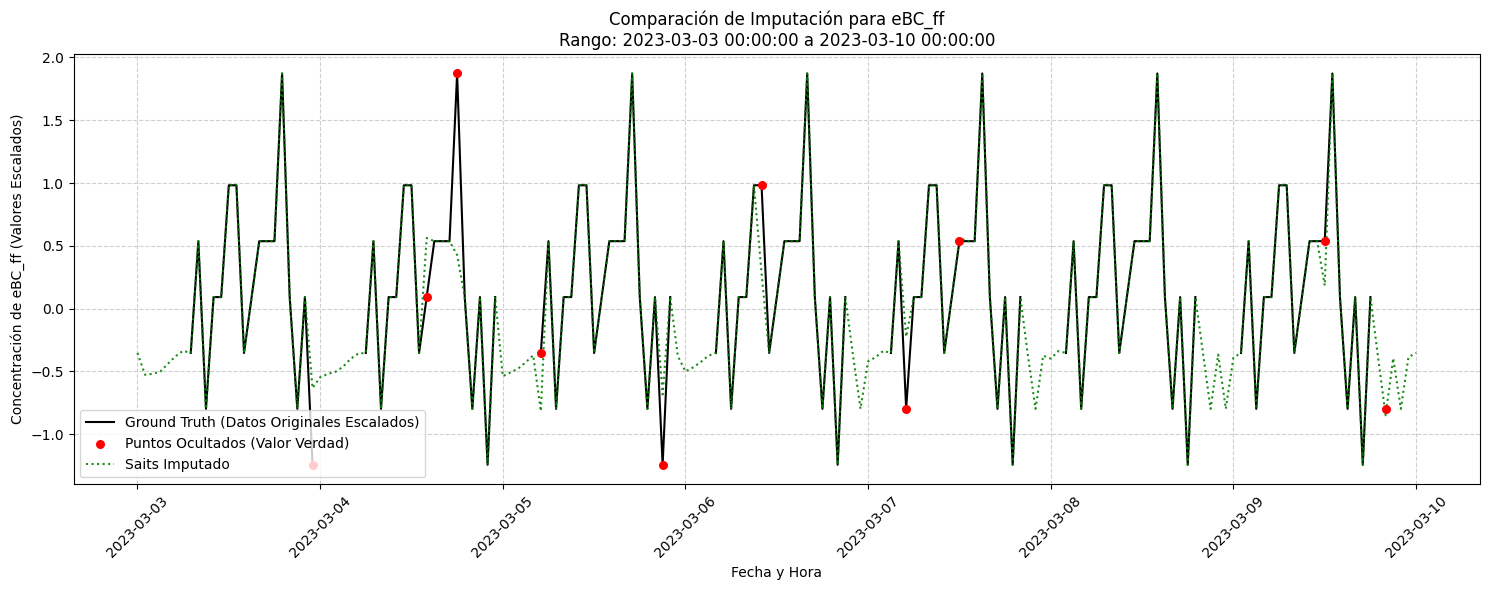
\includegraphics[width=\textwidth]{images/Imputacion/ebc_ff.png}
    \caption{Comparación de imputación para la variable eBC\_ff.}
    \label{fig:imputacion_ebc_ff}
\end{figure}
\begin{figure}[H]
    \centering
    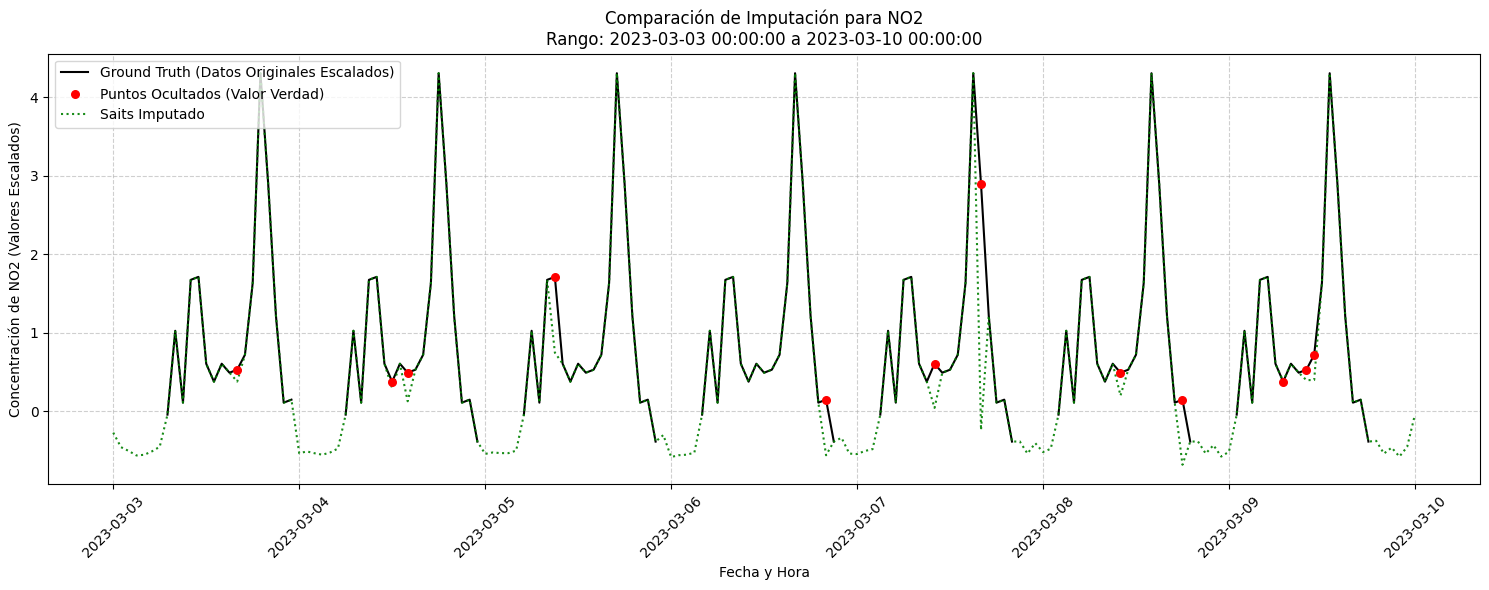
\includegraphics[width=\textwidth]{images/Imputacion/no2.png}
    \caption{Comparación de imputación para la variable NO2.}
    \label{fig:imputacion_no2}
\end{figure}

Eliminar faltantes en las mismas posiciones temporales para todas las variables simplificaría en cierto modo el problema de evaluación, ya que el 'patrón de ausencia' sería el mismo para todas. Al hacerlo de forma independiente, creamos un escenario más complejo y diverso de datos faltantes, lo que nos permite evaluar la generalización del modelo de imputación ante diferentes configuraciones de información disponible.

\begin{figure}[H]
    \centering
    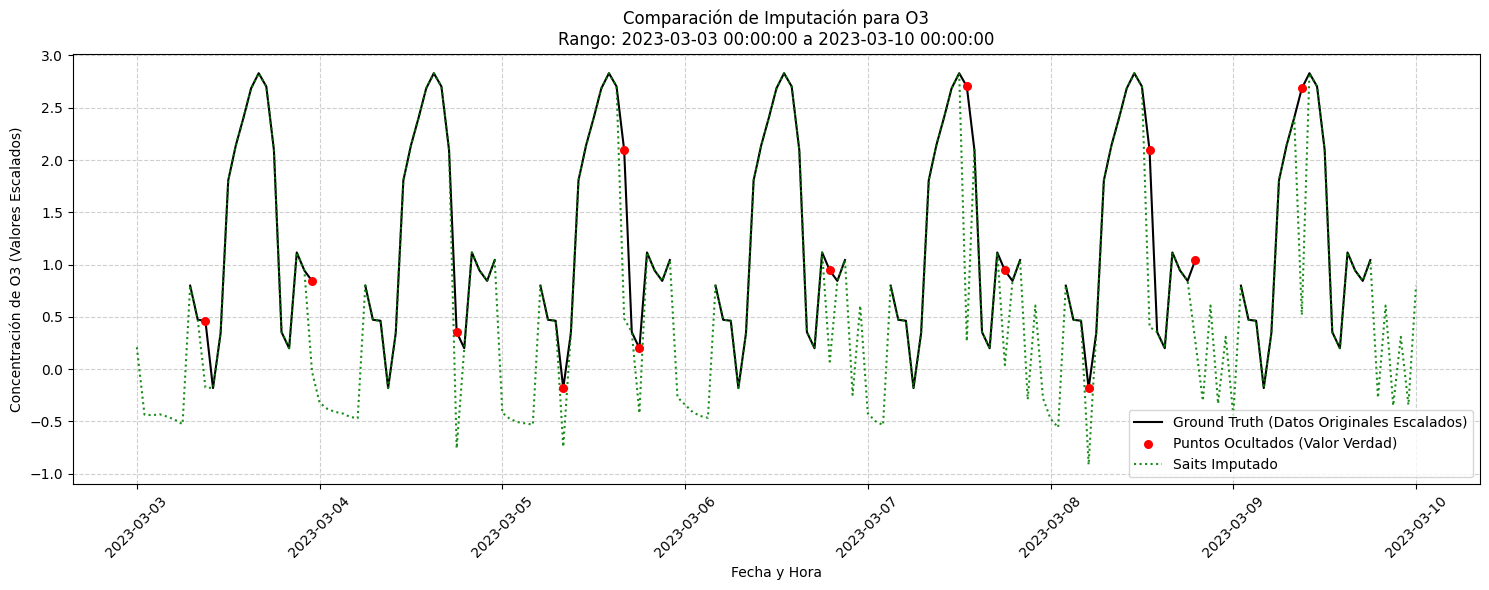
\includegraphics[width=\textwidth]{images/Imputacion/o3.png}
    \caption{Comparación de imputación para la variable O3.}
    \label{fig:imputacion_o3}
\end{figure}

\begin{figure}[H]
    \centering
    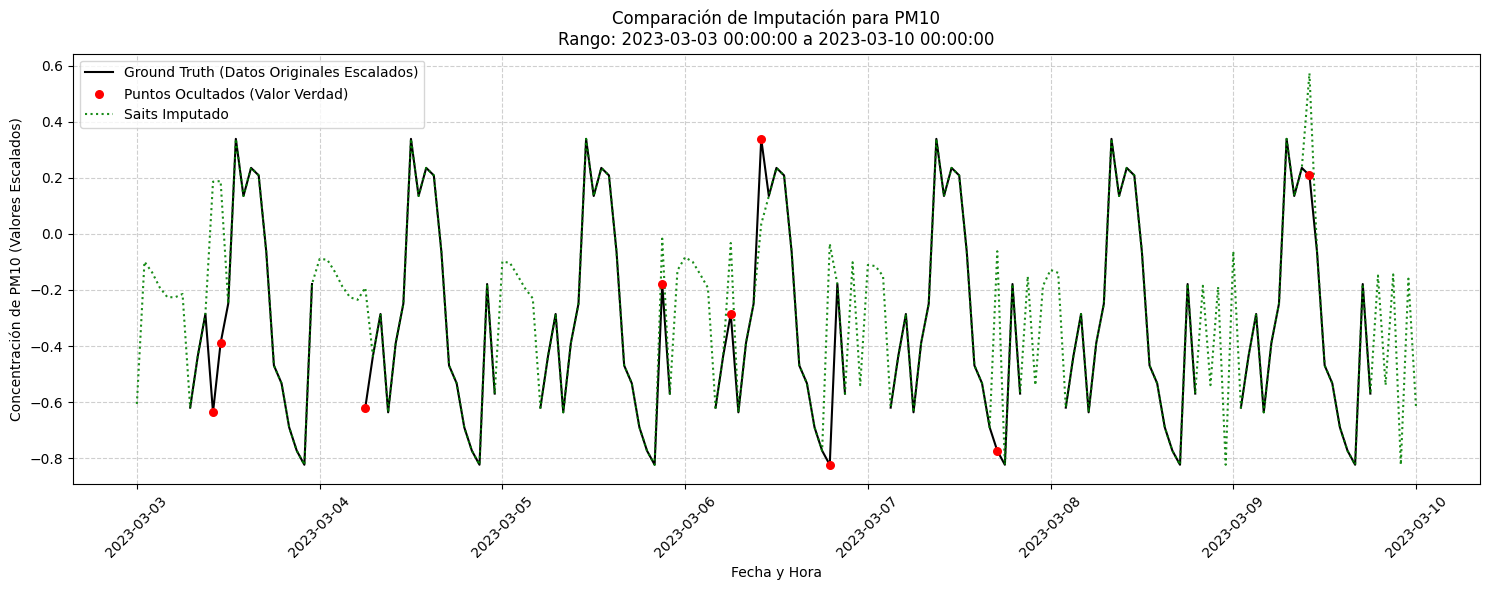
\includegraphics[width=\textwidth]{images/Imputacion/pm10.png}
    \caption{Comparación de imputación para la variable PM10.}
    \label{fig:imputacion_pm10}
\end{figure}

En estas figuras, la línea continua negra representa el \textit{ground truth} (datos originales escalados), los puntos rojos indican los valores que fueron ocultados artificialmente para la prueba del modelo, y la línea punteada verde corresponde a los valores imputados por el modelo \gls{saits}. Se puede observar cómo el modelo de imputación sigue las tendencias generales de los datos originales y la precisión con la que reconstruye los valores en los puntos ocultados.

\section{Evaluación del Rendimiento}
\label{sec:impl_evaluation_summary_revised}
El rendimiento final de cada método se evalúa utilizando el módulo \\ \texttt{pampaneira\_imputation.evaluation}. Este calcula las métricas \gls{mae}, \gls{mse}, \gls{rmse} y \gls{mre} comparando las predicciones $\hat{\mathcal{X}}^{\text{test}}$ con el ground truth $\mathcal{X}_{\text{orig}}^{\text{test}}$ únicamente en las posiciones indicadas por la máscara artificial $\mathbf{M}_{\text{artificial}}^{\text{test}}$.


Las siguientes tablas presentan los resultados de la evaluación de ocho métodos de imputación de datos (Median, Mean, Linear, \gls{ffill}, \gls{bfill}, Hankel, Transformer, \gls{saits}) en dos periodos distintos, utilizando cuatro métricas de error: \gls{rmse}, \gls{mse}, \gls{mae} y \gls{mre}.


\begin{table}[htbp]
\centering
\caption{Resultados de Evaluación - Periodo 1 (10\% ausencia, patrón 'point')}
\label{tab:resultados_periodo1_10_point}
\begin{tabular}{l*{8}{S[table-format=1.4]}} % Se añadió un *8 para 8 columnas de datos
\toprule
\textbf{Métrica} & \textbf{Median} & \textbf{Mean} & \textbf{Linear} & \textbf{Ffill} & \textbf{Bfill} & \textbf{Hankel} & \textbf{Transformer} & \textbf{Saits} \\
\midrule
RMSE & 1.1342 & 1.0521 & 0.8796 & 1.0604 & 1.0487 & 0.8071 & 0.6488 & 0.6360 \\
MSE  & 1.2865 & 1.1069 & 0.7737 & 1.1244 & 1.0997 & 0.6514 & 0.4209 & 0.4045 \\
MAE  & 0.6910 & 0.7346 & 0.4621 & 0.5618 & 0.5554 & 0.5432 & 0.3422 & 0.3263 \\
MRE  & 0.9311 & 0.9898 & 0.6226 & 0.7569 & 0.7484 & 0.7319 & 0.4611 & 0.4397 \\
\bottomrule
\end{tabular}
\end{table}

\begin{figure}[H]
    \centering 
    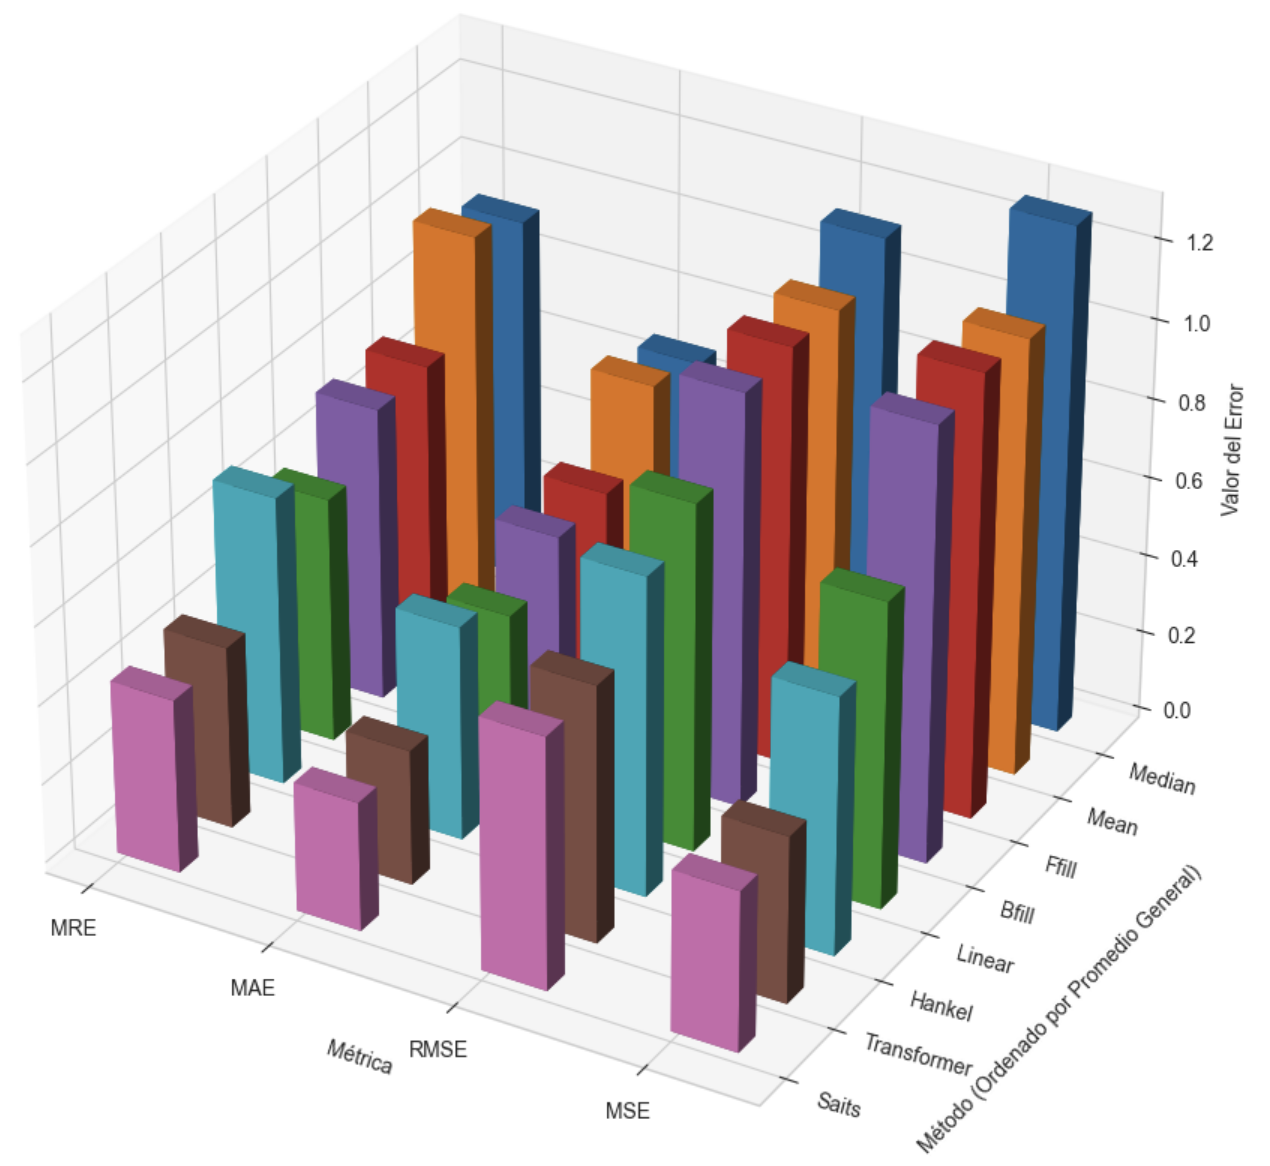
\includegraphics[width=0.8\textwidth]{images/metricas3d_per1.png}
    \caption{Comparativa tridimensional de las métricas de error (\gls{rmse}, \gls{mse}, \gls{mae}, \gls{mre}) para los diferentes métodos de imputación durante el Periodo 1 (10\% ausencia, patrón 'point'). Los métodos están ordenados globalmente según su rendimiento promedio.}
    \label{fig:metricas_3d_periodo1}
\end{figure}

\begin{table}[htbp]
\centering
\caption{Resultados de Evaluación - Periodo 2 (10\% ausencia, patrón 'point')}
\label{tab:resultados_periodo2_10_point}
\begin{tabular}{l*{8}{S[table-format=1.4]}} % Se cambió a *{8} para incluir la columna Hankel
\toprule
\textbf{Métrica} & \textbf{Median} & \textbf{Mean} & \textbf{Linear} & \textbf{Ffill} & \textbf{Bfill} & \textbf{Hankel} & \textbf{Transformer} & \textbf{Saits} \\
\midrule
RMSE & 1.1103 & 1.0609 & 0.9252 & 1.0754 & 1.1018 & 0.8754 & 0.7520 & 0.7428 \\
MSE  & 1.2329 & 1.1255 & 0.8559 & 1.1565 & 1.2140 & 0.7663 & 0.5655 & 0.5517 \\
MAE  & 0.7177 & 0.7637 & 0.4915 & 0.5836 & 0.5894 & 0.5971 & 0.4123 & 0.3980 \\
MRE  & 0.9161 & 0.9747 & 0.6273 & 0.7470 & 0.7544 & 0.7621 & 0.5262 & 0.5079 \\
\bottomrule
\end{tabular}
\end{table}

\begin{figure}[H] 
    \centering 
    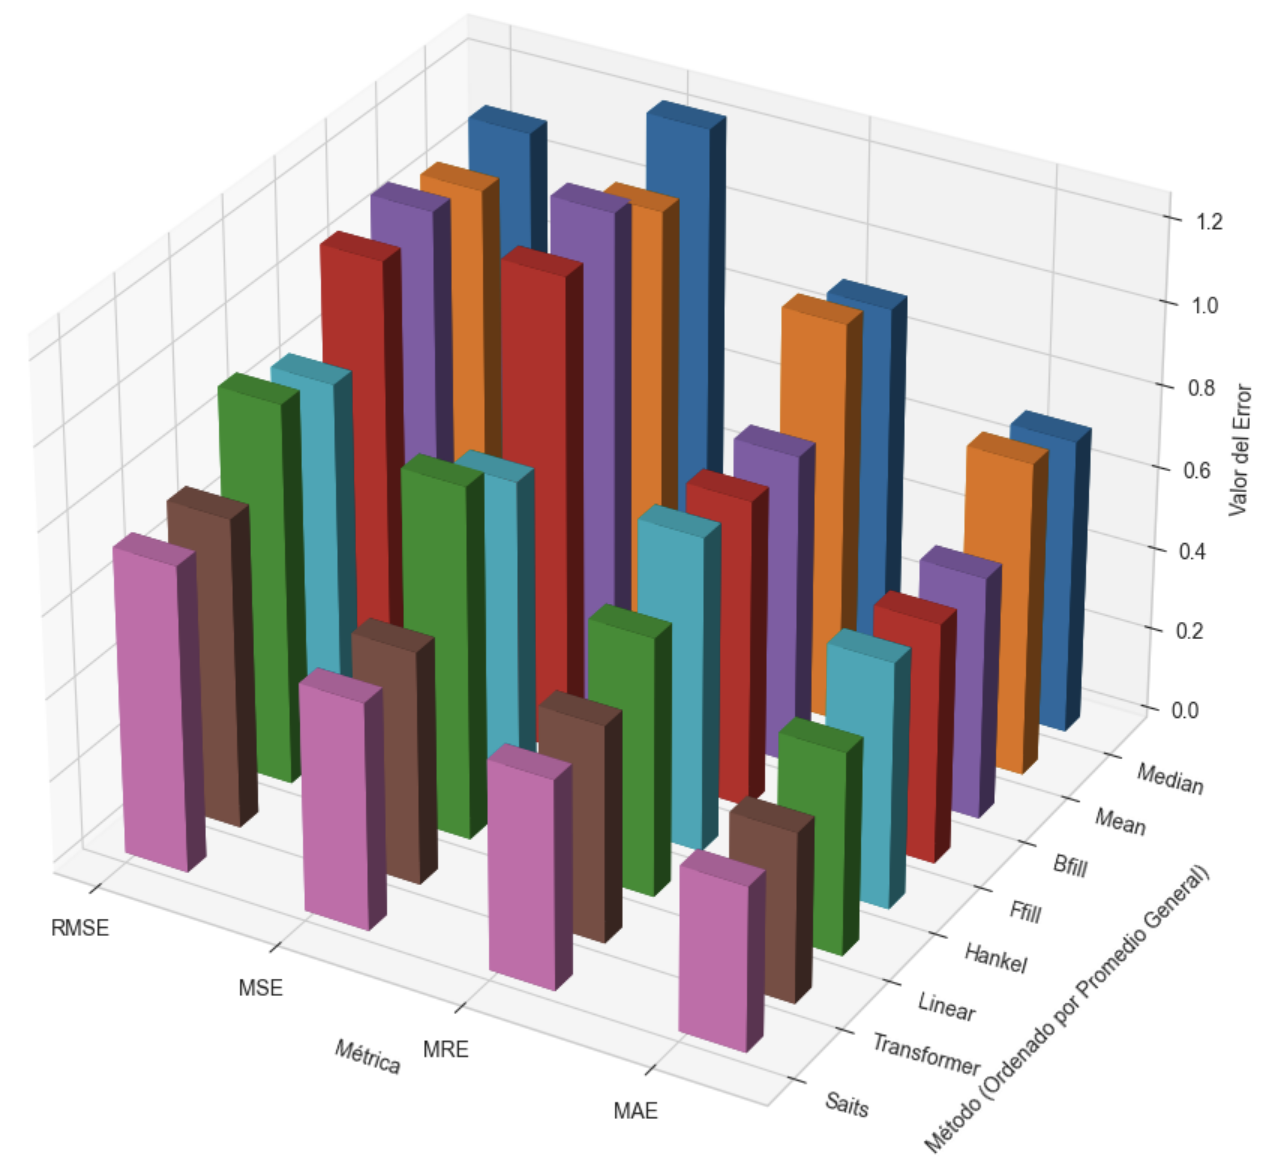
\includegraphics[width=0.8\textwidth]{images/metricas3d_per2.png} 
    \caption{Comparativa tridimensional de las métricas de error (\gls{rmse}, \gls{mse}, \gls{mae}, \gls{mre}) para los diferentes métodos de imputación durante el Periodo 2 (10\% ausencia, patrón 'point'). Los métodos están ordenados globalmente según su rendimiento promedio.}
    \label{fig:metricas_3d_periodo2}
\end{figure}

\subsection*{Nuevos Experimentos con el Dataset de Poqueira}
Para complementar el análisis, se realizaron experimentos adicionales en el dataset de Poqueira, variando el porcentaje de datos faltantes y el patrón de eliminación, permitiendo una evaluación más robusta del comportamiento de los métodos de imputación bajo diferentes condiciones.

\textbf{Experimentos con patrón 'point' (puntual):}
Se introdujeron ausencias artificiales puntuales en los porcentajes del 5\%, 20\% y 50\% de los datos observados.

\begin{table}[htbp]
\centering
\caption{Resultados de Evaluación - Periodo 1 (5\% ausencia, patrón 'point')}
\label{tab:poqueira_5_point_per1}
\begin{tabular}{l*{7}{S[table-format=1.4]}}
\toprule
\textbf{Métrica} & \textbf{Median} & \textbf{Mean} & \textbf{Linear} & \textbf{Ffill} & \textbf{Bfill} & \textbf{Transformer} & \textbf{Saits} \\
\midrule
RMSE & 1.1623 & 1.0886 & 0.9995 & 1.1590 & 1.1588 & 0.6881 & 0.6696 \\
MSE  & 1.3510 & 1.1850 & 0.9989 & 1.3433 & 1.3429 & 0.4735 & 0.4484 \\
MAE  & 0.7142 & 0.7495 & 0.5487 & 0.6480 & 0.6469 & 0.3637 & 0.3504 \\
MRE  & 0.9600 & 1.0075 & 0.7376 & 0.8711 & 0.8696 & 0.4889 & 0.4710 \\
\bottomrule
\end{tabular}
\end{table}

\begin{table}[htbp]
\centering
\caption{Resultados de Evaluación - Periodo 2 (5\% ausencia, patrón 'point')}
\label{tab:poqueira_5_point_per2}
\begin{tabular}{l*{7}{S[table-format=1.4]}}
\toprule
\textbf{Métrica} & \textbf{Median} & \textbf{Mean} & \textbf{Linear} & \textbf{Ffill} & \textbf{Bfill} & \textbf{Transformer} & \textbf{Saits} \\
\midrule
RMSE & 1.1392 & 1.0849 & 1.0187 & 1.1759 & 1.1799 & 0.7628 & 0.7521 \\
MSE  & 1.2977 & 1.1771 & 1.0377 & 1.3828 & 1.3921 & 0.5819 & 0.5657 \\
MAE  & 0.7378 & 0.7736 & 0.5642 & 0.6695 & 0.6668 & 0.4126 & 0.4058 \\
MRE  & 0.9504 & 0.9965 & 0.7268 & 0.8643 & 0.8608 & 0.5316 & 0.5228 \\
\bottomrule
\end{tabular}
\end{table}

\begin{table}[htbp]
\centering
\caption{Resultados de Evaluación - Periodo 1 (20\% ausencia, patrón 'point')}
\label{tab:poqueira_20_point_per1}
\begin{tabular}{l*{7}{S[table-format=1.4]}}
\toprule
\textbf{Métrica} & \textbf{Median} & \textbf{Mean} & \textbf{Linear} & \textbf{Ffill} & \textbf{Bfill} & \textbf{Transformer} & \textbf{Saits} \\
\midrule
RMSE & 1.1440 & 1.0602 & 0.8798 & 1.0541 & 1.0573 & 0.6498 & 0.6415 \\
MSE  & 1.3086 & 1.1240 & 0.7741 & 1.1111 & 1.1179 & 0.4223 & 0.4115 \\
MAE  & 0.6955 & 0.7377 & 0.4568 & 0.5535 & 0.5515 & 0.3364 & 0.3288 \\
MRE  & 0.9302 & 0.9866 & 0.6110 & 0.7403 & 0.7376 & 0.4499 & 0.4397 \\
\bottomrule
\end{tabular}
\end{table}

\begin{table}[htbp]
\centering
\caption{Resultados de Evaluación - Periodo 2 (20\% ausencia, patrón 'point')}
\label{tab:poqueira_20_point_per2}
\begin{tabular}{l*{7}{S[table-format=1.4]}}
\toprule
\textbf{Métrica} & \textbf{Median} & \textbf{Mean} & \textbf{Linear} & \textbf{Ffill} & \textbf{Bfill} & \textbf{Transformer} & \textbf{Saits} \\
\midrule
RMSE & 1.1061 & 1.0589 & 0.9045 & 1.0727 & 1.0736 & 0.7479 & 0.7336 \\
MSE  & 1.2235 & 1.1212 & 0.8181 & 1.1507 & 1.1526 & 0.5593 & 0.5382 \\
MAE  & 0.7187 & 0.7627 & 0.4822 & 0.5783 & 0.5744 & 0.4106 & 0.3896 \\
MRE  & 0.9153 & 0.9713 & 0.6141 & 0.7379 & 0.7330 & 0.5229 & 0.4962 \\
\bottomrule
\end{tabular}
\end{table}

\begin{table}[htbp]
\centering
\caption{Resultados de Evaluación - Periodo 1 (50\% ausencia, patrón 'point')}
\label{tab:poqueira_50_point_per1}
\begin{tabular}{l*{7}{S[table-format=1.4]}}
\toprule
\textbf{Métrica} & \textbf{Median} & \textbf{Mean} & \textbf{Linear} & \textbf{Ffill} & \textbf{Bfill} & \textbf{Transformer} & \textbf{Saits} \\
\midrule
RMSE & 1.1432 & 1.0595 & 0.8994 & 1.0735 & 1.0723 & 0.6606 & 0.6480 \\
MSE  & 1.3070 & 1.1224 & 0.8090 & 1.1524 & 1.1499 & 0.4364 & 0.4199 \\
MAE  & 0.6982 & 0.7369 & 0.4773 & 0.5754 & 0.5746 & 0.3453 & 0.3353 \\
MRE  & 0.9398 & 0.9918 & 0.6425 & 0.7744 & 0.7734 & 0.4647 & 0.4513 \\
\bottomrule
\end{tabular}
\end{table}

\begin{table}[htbp]
\centering
\caption{Resultados de Evaluación - Periodo 2 (50\% ausencia, patrón 'point')}
\label{tab:poqueira_50_point_per2}
\begin{tabular}{l*{7}{S[table-format=1.4]}}
\toprule
\textbf{Métrica} & \textbf{Median} & \textbf{Mean} & \textbf{Linear} & \textbf{Ffill} & \textbf{Bfill} & \textbf{Transformer} & \textbf{Saits} \\
\midrule
RMSE & 1.1172 & 1.0682 & 0.9492 & 1.1078 & 1.1238 & 0.7736 & 0.7508 \\
MSE  & 1.2481 & 1.1411 & 0.9009 & 1.2273 & 1.2629 & 0.5985 & 0.5636 \\
MAE  & 0.7182 & 0.7628 & 0.5055 & 0.6039 & 0.6055 & 0.4157 & 0.3985 \\
MRE  & 0.9192 & 0.9763 & 0.6469 & 0.7746 & 0.7767 & 0.5320 & 0.5100 \\
\bottomrule
\end{tabular}
\end{table}

\clearpage
\textbf{Experimentos con patrón 'subseq' (ráfaga) con longitud entre 8 y 12 horas:}
Se generaron ausencias artificiales en forma de ráfagas de longitud variable (entre 8 y 12 horas) en los porcentajes del 10\%, 20\% y 50\% de los datos observados.

\begin{table}[htbp]
\centering
\caption{Resultados de Evaluación - Periodo 1 (10\% ausencia, patrón 'subseq', longitud 8-12h)}
\label{tab:poqueira_10_subseq_per1}
\begin{tabular}{l*{7}{S[table-format=1.4]}}
\toprule
\textbf{Métrica} & \textbf{Median} & \textbf{Mean} & \textbf{Linear} & \textbf{Ffill} & \textbf{Bfill} & \textbf{Transformer} & \textbf{Saits} \\
\midrule
RMSE & 1.3268 & 1.2476 & 1.2188 & 1.3704 & 1.3628 & 0.6819 & 0.6574 \\
MSE  & 1.7604 & 1.5565 & 1.4855 & 1.8780 & 1.8573 & 0.4650 & 0.4322 \\
MAE  & 0.8666 & 0.8681 & 0.7420 & 0.8574 & 0.8204 & 0.3522 & 0.3370 \\
MRE  & 1.1536 & 1.1556 & 0.9877 & 1.1414 & 1.0922 & 0.4688 & 0.4486 \\
\bottomrule
\end{tabular}
\end{table}

\begin{table}[htbp]
\centering
\caption{Resultados de Evaluación - Periodo 2 (10\% ausencia, patrón 'subseq', longitud 8-12h)}
\label{tab:poqueira_10_subseq_per2}
\begin{tabular}{l*{7}{S[table-format=1.4]}}
\toprule
\textbf{Métrica} & \textbf{Median} & \textbf{Mean} & \textbf{Linear} & \textbf{Ffill} & \textbf{Bfill} & \textbf{Transformer} & \textbf{Saits} \\
\midrule
RMSE & 1.3391 & 1.2408 & 1.1760 & 1.3823 & 1.3831 & 0.7859 & 0.7611 \\
MSE  & 1.7931 & 1.5396 & 1.3830 & 1.9107 & 1.9130 & 0.6176 & 0.5792 \\
MAE  & 0.9164 & 0.8981 & 0.7378 & 0.8742 & 0.8819 & 0.4015 & 0.3890 \\
MRE  & 1.1609 & 1.1376 & 0.9346 & 1.1106 & 1.1204 & 0.5086 & 0.4927 \\
\bottomrule
\end{tabular}
\end{table}

\begin{table}[htbp]
\centering
\caption{Resultados de Evaluación - Periodo 1 (20\% ausencia, patrón 'subseq', longitud 8-12h)}
\label{tab:poqueira_20_subseq_per1}
\begin{tabular}{l*{7}{S[table-format=1.4]}}
\toprule
\textbf{Métrica} & \textbf{Median} & \textbf{Mean} & \textbf{Linear} & \textbf{Ffill} & \textbf{Bfill} & \textbf{Transformer} & \textbf{Saits} \\
\midrule
RMSE & 1.3091 & 1.2399 & 1.2356 & 1.3988 & 1.3624 & 0.6653 & 0.6508 \\
MSE  & 1.7137 & 1.5374 & 1.5266 & 1.9567 & 1.8562 & 0.4427 & 0.4235 \\
MAE  & 0.8541 & 0.8630 & 0.7507 & 0.8736 & 0.8133 & 0.3420 & 0.3299 \\
MRE  & 1.1450 & 1.1569 & 1.0064 & 1.1711 & 1.0903 & 0.4584 & 0.4423 \\
\bottomrule
\end{tabular}
\end{table}

\begin{table}[htbp]
\centering
\caption{Resultados de Evaluación - Periodo 2 (20\% ausencia, patrón 'subseq', longitud 8-12h)}
\label{tab:poqueira_20_subseq_per2}
\begin{tabular}{l*{7}{S[table-format=1.4]}}
\toprule
\textbf{Métrica} & \textbf{Median} & \textbf{Mean} & \textbf{Linear} & \textbf{Ffill} & \textbf{Bfill} & \textbf{Transformer} & \textbf{Saits} \\
\midrule
RMSE & 1.3342 & 1.2423 & 1.2161 & 1.3747 & 1.3931 & 0.8019 & 0.7838 \\
MSE  & 1.7801 & 1.5432 & 1.4789 & 1.8899 & 1.9406 & 0.6430 & 0.6144 \\
MAE  & 0.9074 & 0.8944 & 0.7614 & 0.8757 & 0.8853 & 0.4247 & 0.4054 \\
MRE  & 1.1687 & 1.1520 & 0.9806 & 1.1291 & 1.1415 & 0.5470 & 0.5222 \\
\bottomrule
\end{tabular}
\end{table}

\begin{table}[htbp]
\centering
\caption{Resultados de Evaluación - Periodo 1 (50\% ausencia, patrón 'subseq', longitud 8-12h)}
\label{tab:poqueira_50_subseq_per1}
\begin{tabular}{l*{7}{S[table-format=1.4]}}
\toprule
\textbf{Métrica} & \textbf{Median} & \textbf{Mean} & \textbf{Linear} & \textbf{Ffill} & \textbf{Bfill} & \textbf{Transformer} & \textbf{Saits} \\
\midrule
RMSE & 1.2944 & 1.2242 & 1.2103 & 1.3939 & 1.3535 & 0.6743 & 0.6581 \\
MSE  & 1.6755 & 1.4986 & 1.4647 & 1.9430 & 1.8319 & 0.4546 & 0.4332 \\
MAE  & 0.8500 & 0.8590 & 0.7374 & 0.8662 & 0.8090 & 0.3518 & 0.3459 \\
MRE  & 1.1430 & 1.1551 & 0.9917 & 1.1648 & 1.0880 & 0.4731 & 0.4652 \\
\bottomrule
\end{tabular}
\end{table}

\begin{table}[htbp]
\centering
\caption{Resultados de Evaluación - Periodo 2 (50\% ausencia, patrón 'subseq', longitud 8-12h)}
\label{tab:poqueira_50_subseq_per2}
\begin{tabular}{l*{7}{S[table-format=1.4]}}
\toprule
\textbf{Métrica} & \textbf{Median} & \textbf{Mean} & \textbf{Linear} & \textbf{Ffill} & \textbf{Bfill} & \textbf{Transformer} & \textbf{Saits} \\
\midrule
RMSE & 1.3032 & 1.2123 & 1.1853 & 1.3597 & 1.3595 & 0.7713 & 0.7530 \\
MSE  & 1.6982 & 1.4696 & 1.4049 & 1.8489 & 1.8482 & 0.5950 & 0.5671 \\
MAE  & 0.8943 & 0.8846 & 0.7500 & 0.8656 & 0.8673 & 0.4150 & 0.4021 \\
MRE  & 1.1591 & 1.1465 & 0.9720 & 1.1240 & 1.1261 & 0.5379 & 0.5212 \\
\bottomrule
\end{tabular}
\end{table}

\clearpage
\subsubsection*{Visualizaciones de PM10 para los nuevos experimentos en Poqueira}

\begin{figure}[H]
    \centering
    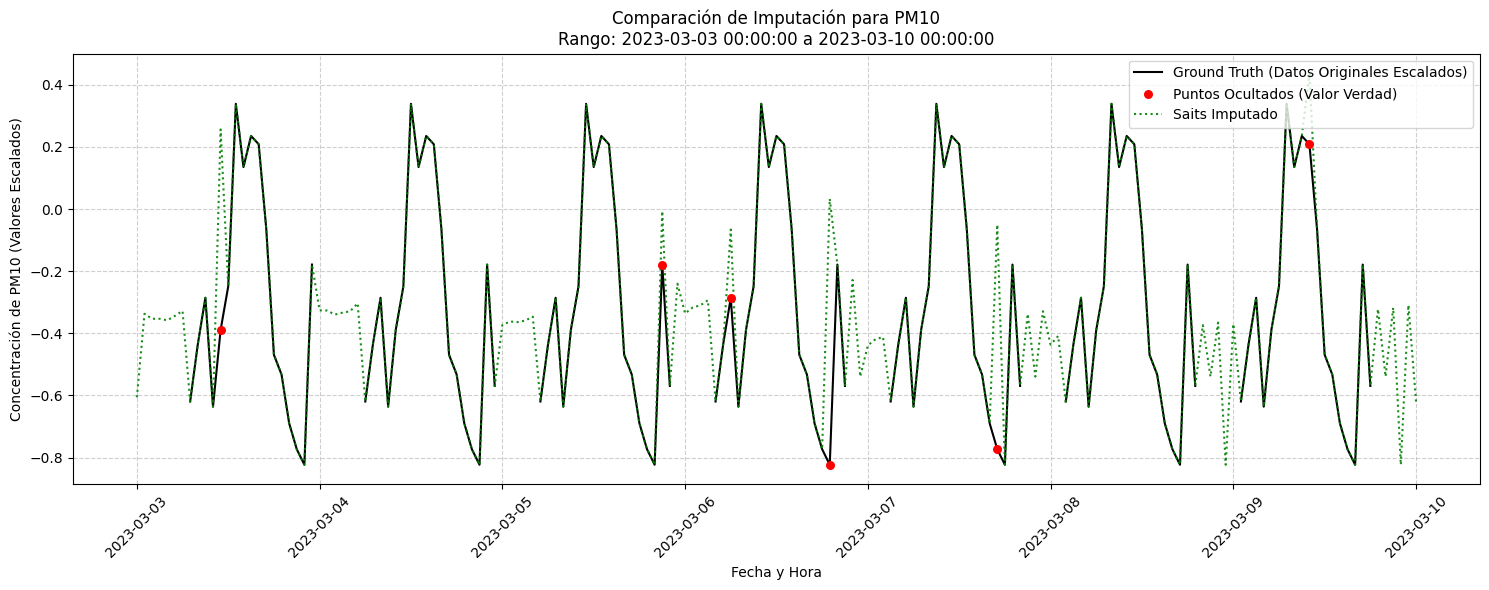
\includegraphics[width=\textwidth]{images/pm10_5_point.png}
    \caption{Comparación de imputación para la variable PM10 en Poqueira (5\% ausencia, patrón 'point', Periodo 2).}
    \label{fig:pm10_5_point}
\end{figure}
\begin{figure}[H]
    \centering
    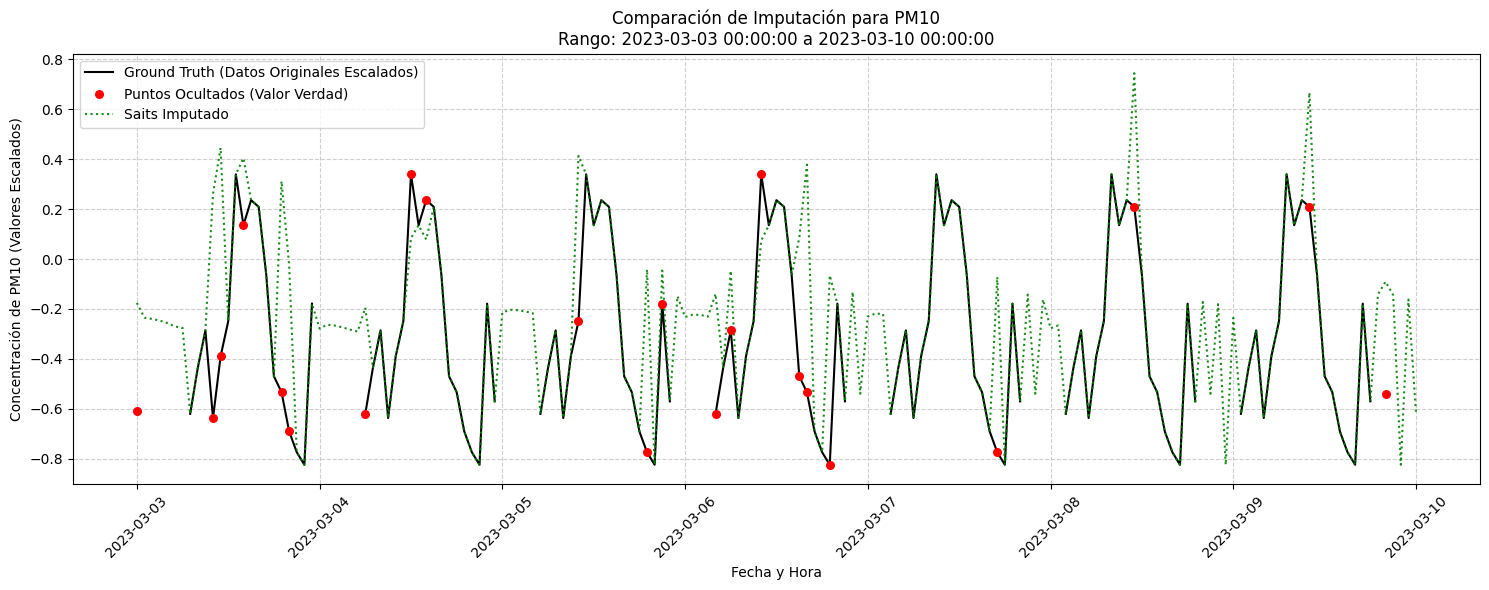
\includegraphics[width=\textwidth]{images/pm10_20_point.png}
    \caption{Comparación de imputación para la variable PM10 en Poqueira (20\% ausencia, patrón 'point', Periodo 2).}
    \label{fig:pm10_20_point}
\end{figure}

\begin{figure}[H]
    \centering
    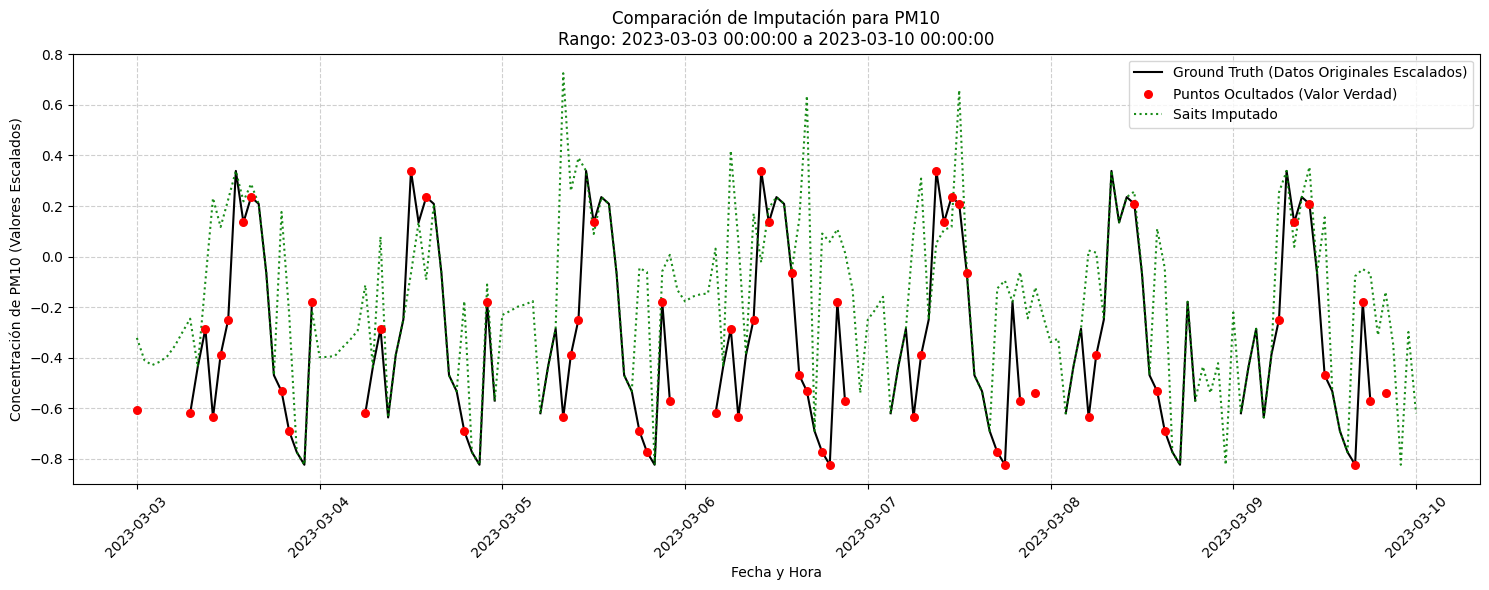
\includegraphics[width=\textwidth]{images/pm10_50_point.png}
    \caption{Comparación de imputación para la variable PM10 en Poqueira (50\% ausencia, patrón 'point', Periodo 2).}
    \label{fig:pm10_20_point}
\end{figure}
\begin{figure}[H]
    \centering
    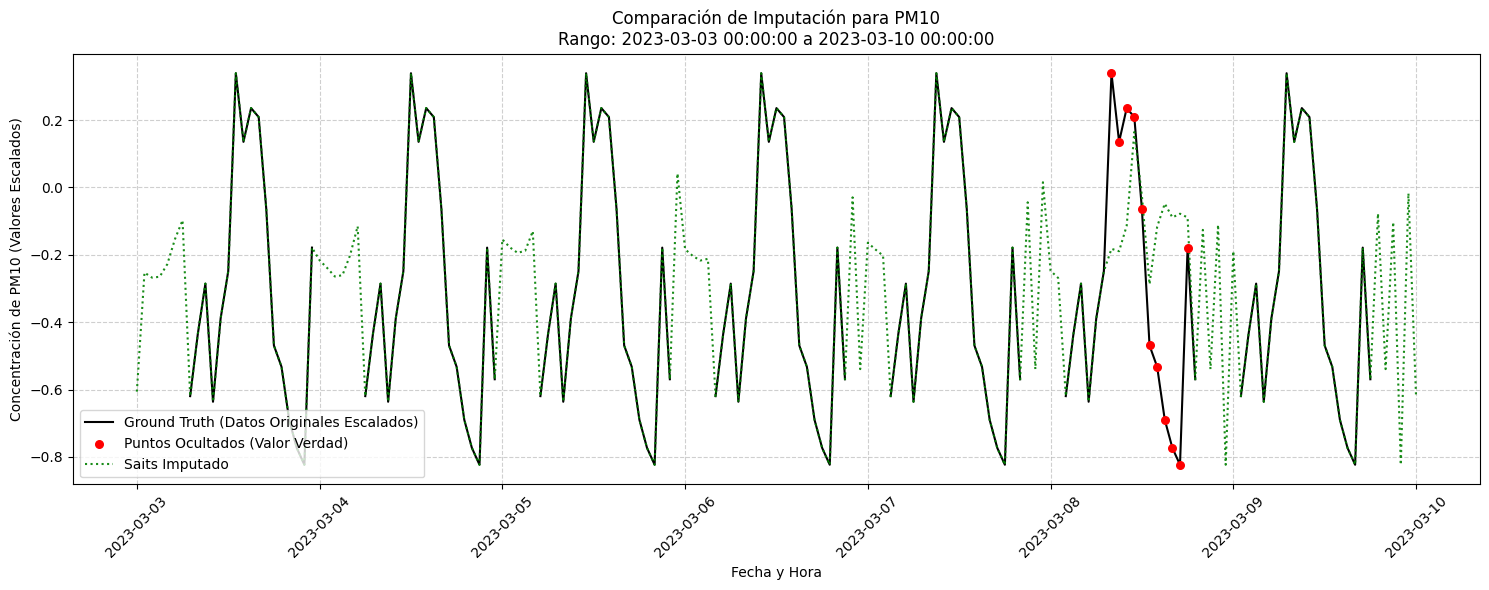
\includegraphics[width=\textwidth]{images/pm10_10_subseq.png}
    \caption{Comparación de imputación para la variable PM10 en Poqueira (10\% ausencia, patrón 'subseq', longitud 8-12h, Periodo 2).}
    \label{fig:pm10_10_subseq}
\end{figure}

\begin{figure}[H]
    \centering
    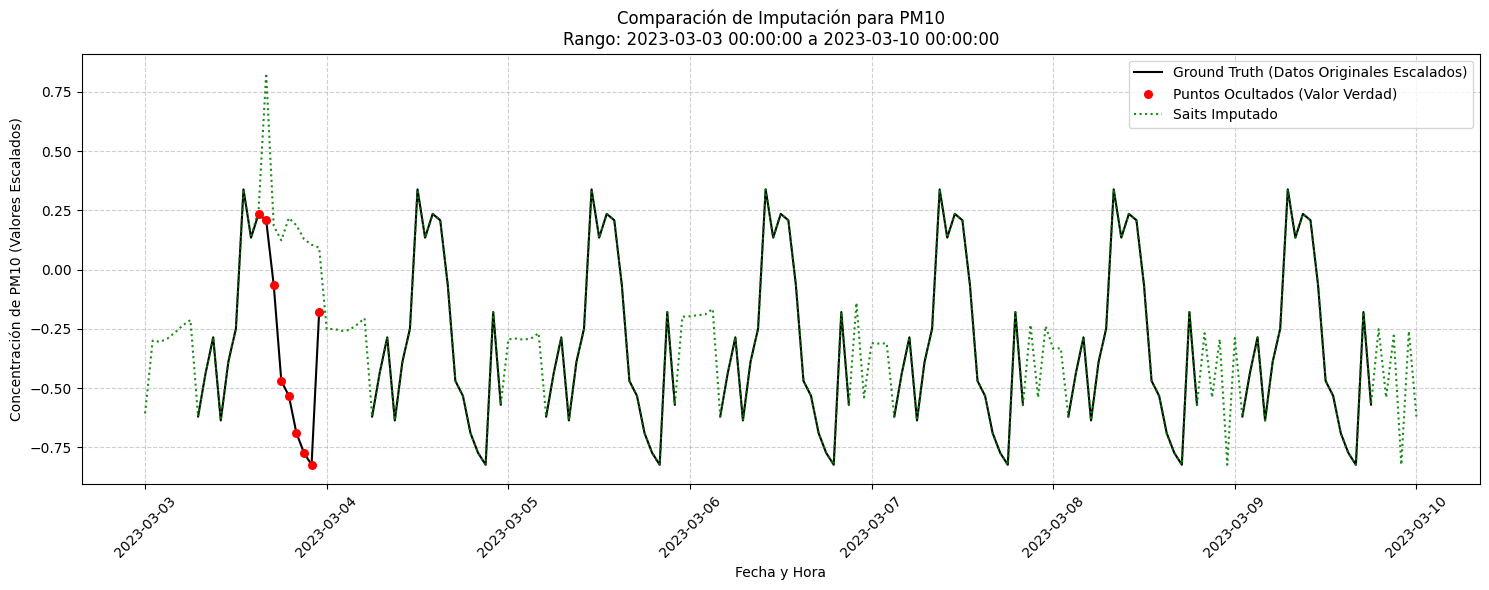
\includegraphics[width=\textwidth]{images/pm10_20_subseq.png}
    \caption{Comparación de imputación para la variable PM10 en Poqueira (20\% ausencia, patrón 'subseq', longitud 8-12h, Periodo 2).}
    \label{fig:pm_10_20_subseq}
\end{figure}
\begin{figure}[H]
    \centering
    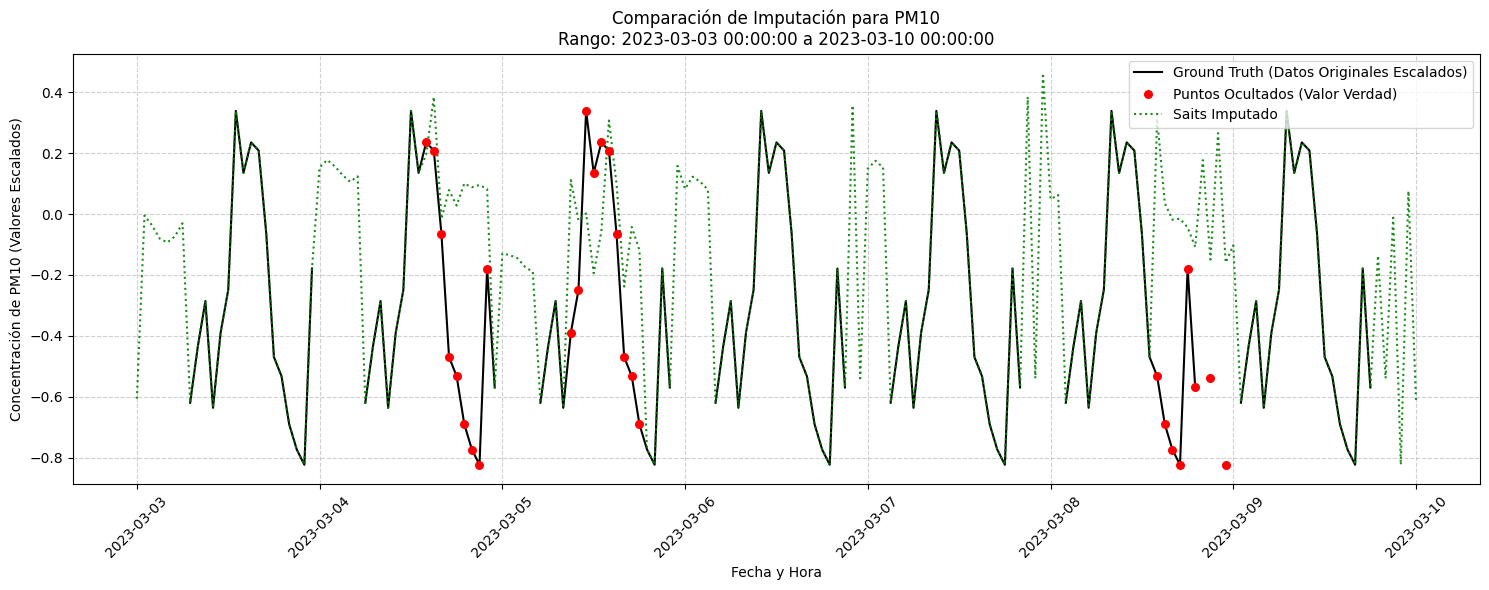
\includegraphics[width=\textwidth]{images/pm10_50_subseq.png}
    \caption{Comparación de imputación para la variable PM10 en Poqueira (50\% ausencia, patrón 'subseq', longitud 8-12h, Periodo 2).}
    \label{fig:pm10_50_subseq}
\end{figure}

\section*{Interpretación de los Resultados}

 Para todas estas métricas, \textbf{valores más bajos indican un mejor rendimiento} del método de imputación, ya que representan un menor error entre los valores imputados y los valores reales.

\subsection*{Discusión General del Rendimiento de los Métodos}

\begin{itemize}
    \item \textbf{Rendimiento de los Métodos Básicos y Tradicionales:}
    Los enfoques más elementales como la imputación por \textbf{Mean} y \textbf{Median} registraron consistentemente los errores más elevados, demostrando una limitada capacidad para inferir datos faltantes con precisión. Los métodos de propagación, \textbf{\gls{ffill}} y \textbf{\gls{bfill}}, exhibieron un rendimiento inconsistente y variable, siendo sensibles a la posición de los datos faltantes en la secuencia. Entre los métodos tradicionales más simples, la imputación \textbf{Linear} (interpolación lineal) se mostró como la más efectiva, superando a los enfoques basados en media, mediana y propagación en la mayoría de los escenarios.

    \item \textbf{Imputación Hankel (HI): Un Intermedio Eficaz:}
    La \textbf{Imputación Hankel}, un método basado en la completación de matrices de bajo rango, se destacó por ofrecer un rendimiento notablemente superior al de los métodos básicos (Mean, Median, Ffill, Bfill) y a la interpolación lineal (Linear). Para el escenario de 10\% de ausencia puntual, tanto en el Periodo 1 (Cuadro \ref{tab:poqueira_5_point_per1}) como en el Periodo 2 (Cuadro \ref{tab:poqueira_50_point_per2}), \textbf{Imputación Hankel} mostró errores significativamente menores que Linear en todas las métricas, posicionándose claramente como el tercer método más preciso. Este resultado sugiere que la Imputación Hankel es capaz de capturar eficazmente las dependencias temporales y la estructura subyacente de la serie, lo que le permite imputar valores con una alta fidelidad comparado con los enfoques más simples.

    \item \textbf{Dominio Absoluto de Modelos Predictivos Avanzados:}
    Los modelos basados en arquitecturas Transformer, específicamente \textbf{\gls{saits}} y \textbf{Transformer}, demostraron consistentemente una precisión superior en la imputación de datos faltantes en comparación con todos los demás métodos, incluidos los tradicionales y la Imputación Hankel. Esto se reflejó en errores notablemente inferiores en todas las métricas y en ambos periodos de estudio. Dentro de este grupo de modelos avanzados, \textbf{\gls{saits}} se destacó por ofrecer el rendimiento más preciso de manera generalizada, obteniendo los errores más bajos en la mayoría de las evaluaciones, aunque seguido de cerca por el modelo \textbf{Transformer}. Su capacidad para modelar dependencias a largo plazo y aprender representaciones complejas de los datos les otorgó una ventaja decisiva en la reconstrucción de información faltante, estableciendo un claro liderazgo en la jerarquía de precisión.
    
\end{itemize}

\subsection*{Análisis Comparativo entre Periodos de Estudio}

\begin{itemize}
    \item \textbf{Variación del Error entre Periodos:} Se observó una tendencia general hacia errores de imputación ligeramente mayores durante el Periodo 2 en comparación con el Periodo 1 para la mayoría de los métodos, especialmente los de mejor rendimiento. Esto incluyó a la \textbf{Imputación Hankel}, cuyo error, si bien se mantuvo muy bajo, también mostró un ligero incremento. Esta diferencia podría deberse a que el Periodo 2 es mucho más reducido, limitando la cantidad de datos para la inferencia.

    \item \textbf{Estabilidad en la Jerarquía de Métodos:} A pesar de las fluctuaciones en los niveles de error absoluto entre los dos periodos, la jerarquía de rendimiento relativo entre los modelos se mantuvo en gran medida estable. Los modelos \textbf{\gls{saits}} y \textbf{Transformer} continuaron siendo los más precisos, seguidos consistentemente por la \textbf{Imputación Hankel}, la cual mantuvo su sólida posición como el tercer método más preciso, confirmando su robustez y fiabilidad frente a los métodos más simples.
\end{itemize}

\subsection*{Observaciones Clave por Tipo de Métrica de Error}
\begin{itemize}
    \item \textbf{Impacto de Errores Grandes (\gls{rmse} y \gls{mse}):} Las métricas que magnifican el impacto de errores grandes, como \gls{rmse} y \gls{mse}, confirmaron la robustez de \textbf{\gls{saits}}, \textbf{Transformer} y la \textbf{Imputación Hankel}. Sus bajos valores en estas métricas sugieren que estos modelos no solo son precisos en promedio, sino que también son menos propensos a cometer errores de gran magnitud.
    \item \textbf{Error Promedio Absoluto (\gls{mae}):} El \gls{mae}, que mide la desviación promedio absoluta, también resaltó la superioridad de \textbf{\gls{saits}}, \textbf{Transformer} y la \textbf{Imputación Hankel}, indicando que sus imputaciones se encuentran, en promedio, más próximas a los valores verdaderos.
    \item \textbf{Error Relativo (\gls{mre}):} Al considerar el error desde una perspectiva porcentual a través del \gls{mre}, se reafirmó la mayor precisión de los modelos \textbf{\gls{saits}}, \textbf{Transformer} y la \textbf{Imputación Hankel} en comparación con los otros métodos evaluados.
\end{itemize}

\subsection*{Análisis de los Resultados en el Dataset de Poqueira bajo diferentes escenarios}
Se evaluaron los métodos de imputación con diferentes porcentajes de ausencia (5\%, 10\%, 20\%, 50\%) y patrones ('point' y 'subseq' con longitud 8-12h).

\begin{itemize}
    \item \textbf{Impacto del Porcentaje de Datos Faltantes (Patrón 'point'):}
    Al aumentar el porcentaje de datos faltantes (de 5\% a 50\%) con el patrón 'point' (Tablas \ref{tab:poqueira_5_point_per1} a \ref{tab:poqueira_50_point_per2}), se observa una tendencia general al \textbf{incremento de los errores} para todos los métodos. Esto es esperado, ya que una mayor cantidad de datos ausentes reduce la información disponible para realizar imputaciones precisas. Sin embargo, los modelos avanzados (Transformer y \gls{saits}) mantienen su superioridad, mostrando un aumento de error más moderado en comparación con los métodos tradicionales, lo que subraya su robustez ante escenarios con mayor escasez de datos.

    \item \textbf{Impacto del Patrón de Ausencia ('point' vs. 'subseq'):}
    Al comparar los resultados para un mismo porcentaje de ausencia (por ejemplo, 10\%, 20\%, 50\%) pero con diferentes patrones (Tablas \ref{tab:resultados_periodo1_10_point}/\ref{tab:resultados_periodo2_10_point} vs. \ref{tab:poqueira_10_subseq_per1}/\ref{tab:poqueira_10_subseq_per2}), se observa que el patrón 'subseq' generalmente resulta en \textbf{errores mayores} para todos los métodos. Las ráfagas de datos faltantes (subsecuencias) representan un desafío mayor que las ausencias puntuales, ya que la información temporal contigua es más limitada. En este escenario más complejo, la ventaja de los modelos Transformer y \gls{saits} se hace aún más pronunciada, demostrando su capacidad para capturar dependencias a largo plazo y reconstruir secuencias completas de datos faltantes de manera más efectiva que los métodos simples. El método Linear, aunque mejor que Mean/Median/Ffill/Bfill en el patrón 'point', también ve su rendimiento deteriorarse significativamente con 'subseq' en comparación con los modelos avanzados.

    \item \textbf{Rendimiento de los Métodos Tradicionales:}
    Los métodos como Median, Mean, \gls{ffill} y \gls{bfill} muestran un rendimiento consistentemente inferior, especialmente a medida que la proporción de datos faltantes o la complejidad del patrón de ausencia aumenta. Su dependencia de información local o agregada simple los hace menos efectivos para inferir valores en series temporales con patrones complejos o extensos periodos de ausencia.

\end{itemize}

%%%%.

\section{Validación en otro dataset de contaminación de la literatura}

Para complementar las pruebas con datos de Poqueira y validar la capacidad de SAITS en un benchmark reconocido, se realizó un experimento adicional con el conjunto de datos de calidad del aire de Beijing (Air-Quality) \citep[cf.][]{Du2023SAITS}. Este dataset incluye datos horarios de contaminantes atmosféricos de 12 sitios de monitoreo en Beijing, recopilados durante 48 meses (marzo de 2013 a febrero de 2017), resultando en 132 variables de características. Originalmente presenta una tasa de valores faltantes del 1.6\%, y para la evaluación controlada del rendimiento de los modelos, se generaron ausencias artificiales \textbf{puntuales} en el 10\% de los valores observados. Este experimento, que replicó parte de la metodología del estudio de referencia, tuvo como objetivo demostrar la eficacia del modelo en un contexto externo. Los resultados obtenidos para las métricas de error, registrados en la \Cref{tab:resultados_pekin_eval}, confirman el desempeño superior de los modelos basados en autoatención. El \textbf{Jupyter Notebook\footnote{\url{https://github.com/eigenric/TFG/blob/main/notebooks/Notebook_Pekin.ipynb}}} se encuentra disponible en el repositorio de Github.

% --- Aquí va la tabla LaTeX con los resultados del dataset de Beijing ---
\begin{table}[htbp]
\centering
\caption{Resultados de Evaluación - Dataset Air-Quality de Beijing (10\% ausencia, patrón 'point')}
\label{tab:resultados_pekin_eval}
\begin{tabular}{l*{5}{S[table-format=1.4]}}
\toprule
\textbf{Métrica} & \textbf{Median} & \textbf{Mean} & \textbf{Ffill} & \textbf{Transformer} & \textbf{Saits} \\
\midrule
RMSE & 0.6435 & 0.6170 & 0.5493 & 0.5320 & 0.5156 \\
MSE  & 0.4141 & 0.3806 & 0.3018 & 0.2831 & 0.2659 \\
MAE  & 0.3116 & 0.3202 & 0.1896 & 0.1940 & 0.1793 \\
MRE  & 0.4145 & 0.4259 & 0.2517 & 0.2580 & 0.2385 \\
\bottomrule
\end{tabular}
\end{table}


\begin{figure}[H] 
    \centering 
    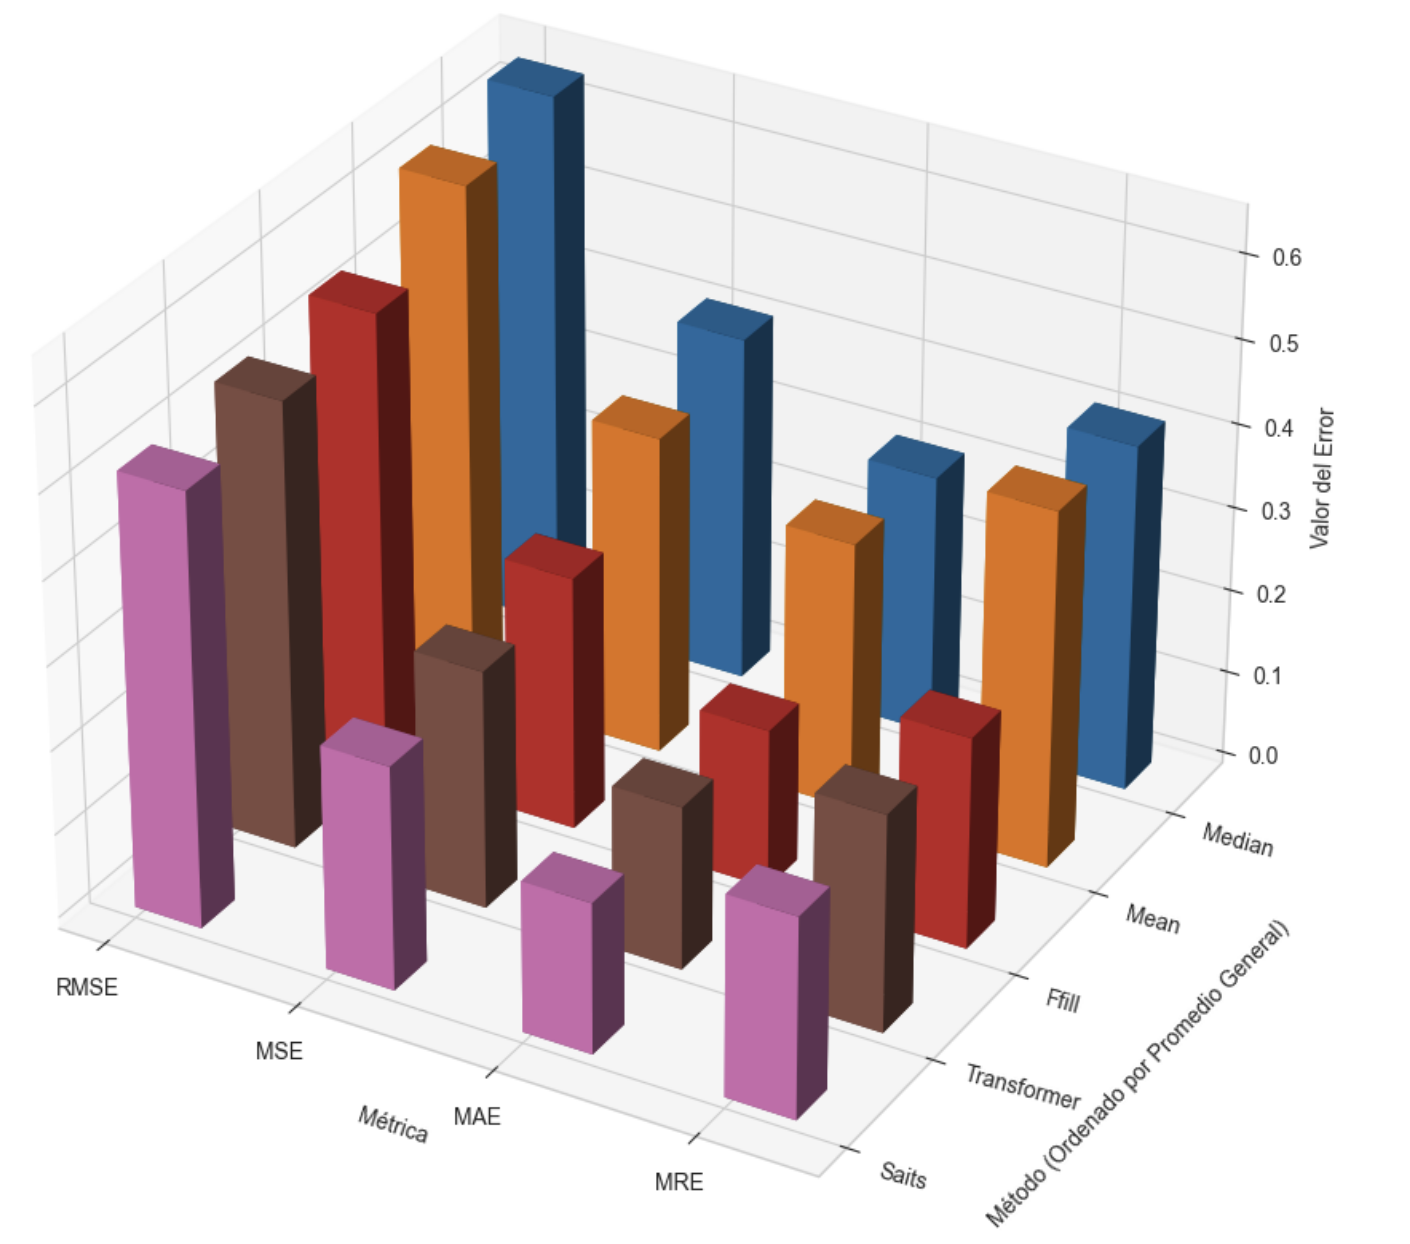
\includegraphics[width=0.8\textwidth]{images/metricas3d_pekin.png} 
    \caption{Comparativa tridimensional de las métricas de error para los diferentes métodos de imputación 
    en el Dataset de Air-Quality de Beijing. }
    \label{fig:metricas_3d_periodo1}
\end{figure}

Extendiendo el análisis de patrones de ausencia, se evaluaron dos configuraciones adicionales para el dataset de calidad del aire de Beijing, utilizando un patrón de eliminación por \textbf{ráfaga ('subseq')} para secuencias de 5 horas, con porcentajes de datos faltantes del 20\% y 50\%. Los resultados se presentan en las \Cref{tab:resultados_pekin_eval_20_subseq_5} y \Cref{tab:resultados_pekin_eval_50_subseq_5} respectivamente.

\begin{itemize}
    \item \textbf{Impacto del Porcentaje de Datos Faltantes:}
    Al comparar los resultados de los patrones de ráfaga con longitud 5 (Tablas \ref{tab:resultados_pekin_eval_20_subseq_5} y \ref{tab:resultados_pekin_eval_50_subseq_5}), se observa una clara tendencia: a medida que el porcentaje de datos faltantes aumenta del 20\% al 50\%, todas las métricas de error para todos los métodos tienden a \textbf{incrementar}. Esto es esperable, ya que una mayor escasez de información reduce la capacidad de inferencia. Sin embargo, los modelos \glsentryshort{transformer} y \glsentryshort{saits} consistentemente mantienen los errores más bajos en comparación con los métodos tradicionales.

    \item \textbf{Rendimiento de los Métodos ante el Patrón 'Subseq':}
    Bajo el patrón de eliminación 'subseq', los modelos Transformer y SAITS continúan demostrando una superioridad significativa en todas las métricas. La imputación por ffill muestra un rendimiento competitivo frente a la mediana y la media en este tipo de patrón estructurado, y en algunos casos supera incluso a la media. Como es común, los métodos simples como la mediana y la  media registran los errores más elevados, reflejando su limitada capacidad para manejar patrones de ausencia complejos.
\end{itemize}

% --- TABLA: 20% Faltantes, Patrón Subseq, Longitud 5 ---
\begin{table}[htbp]
\centering
\caption{Resultados de Evaluación - Dataset Air-Quality de Beijing (20\% Faltantes, Patrón Subseq, Longitud 5)}
\label{tab:resultados_pekin_eval_20_subseq_5}
\begin{tabular}{l*{5}{S[table-format=1.4]}}
\toprule
\textbf{Métrica} & \textbf{Median} & \textbf{Mean} & \textbf{Ffill} & \textbf{Transformer} & \textbf{Saits} \\
\midrule
RMSE & 0.6891 & 0.6374 & 0.6971 & 0.4827 & 0.4710 \\
MSE  & 0.4749 & 0.4063 & 0.4860 & 0.2330 & 0.2219 \\
MAE  & 0.3643 & 0.3588 & 0.3009 & 0.1961 & 0.1827 \\
MRE  & 0.4845 & 0.4772 & 0.3991 & 0.2608 & 0.2429 \\
\bottomrule
\end{tabular}
\end{table}

% --- TABLA: 50% Faltantes, Patrón Bloque, Longitud 5 ---
\begin{table}[htbp]
\centering
\caption{Resultados de Evaluación - Dataset Air-Quality de Beijing (50\% Faltantes, Patrón Subseq, Longitud 5)}
\label{tab:resultados_pekin_eval_50_subseq_5}
\begin{tabular}{l*{5}{S[table-format=1.4]}}
\toprule
\textbf{Métrica} & \textbf{Median} & \textbf{Mean} & \textbf{Ffill} & \textbf{Transformer} & \textbf{Saits} \\
\midrule
RMSE & 0.7945 & 0.7506 & 0.7778 & 0.6385 & 0.6254 \\
MSE  & 0.6313 & 0.5635 & 0.6050 & 0.4076 & 0.3911 \\
MAE  & 0.3770 & 0.3696 & 0.3605 & 0.2167 & 0.2021 \\
MRE  & 0.4981 & 0.4883 & 0.4752 & 0.2864 & 0.2670 \\
\bottomrule
\end{tabular}
\end{table}